\chapter{Results and Evaluation}\label{ch: results and eval}
In this chapter we present our experimental results and their corresponding evaluation. Our experiment was built to evaluate whether DC Transformation helps improve model performance in univariate time series forecasting. Our experiment covers weekly, daily, and hourly frequencies and the results are investigated separately based on the performance metrics we addressed in Section \ref{subsec: performance metrics}. For a model `M', agents using model `M' without DC Transformation are named `M\_raw' and agents using model `M' with DC Transformation are named `M\_tran'.

\section{Analysing Weekly Time Series}
We start by looking at the weekly financial time series and the summary statistics of the agents. Figure \ref{fig: weekly smape box} shows that the agents have about the same level of overall performance across the time series tested. In addition, agents with and without DC Transformation do not generate different ranges of errors in general.
\begin{figure}[H]
    \centering
    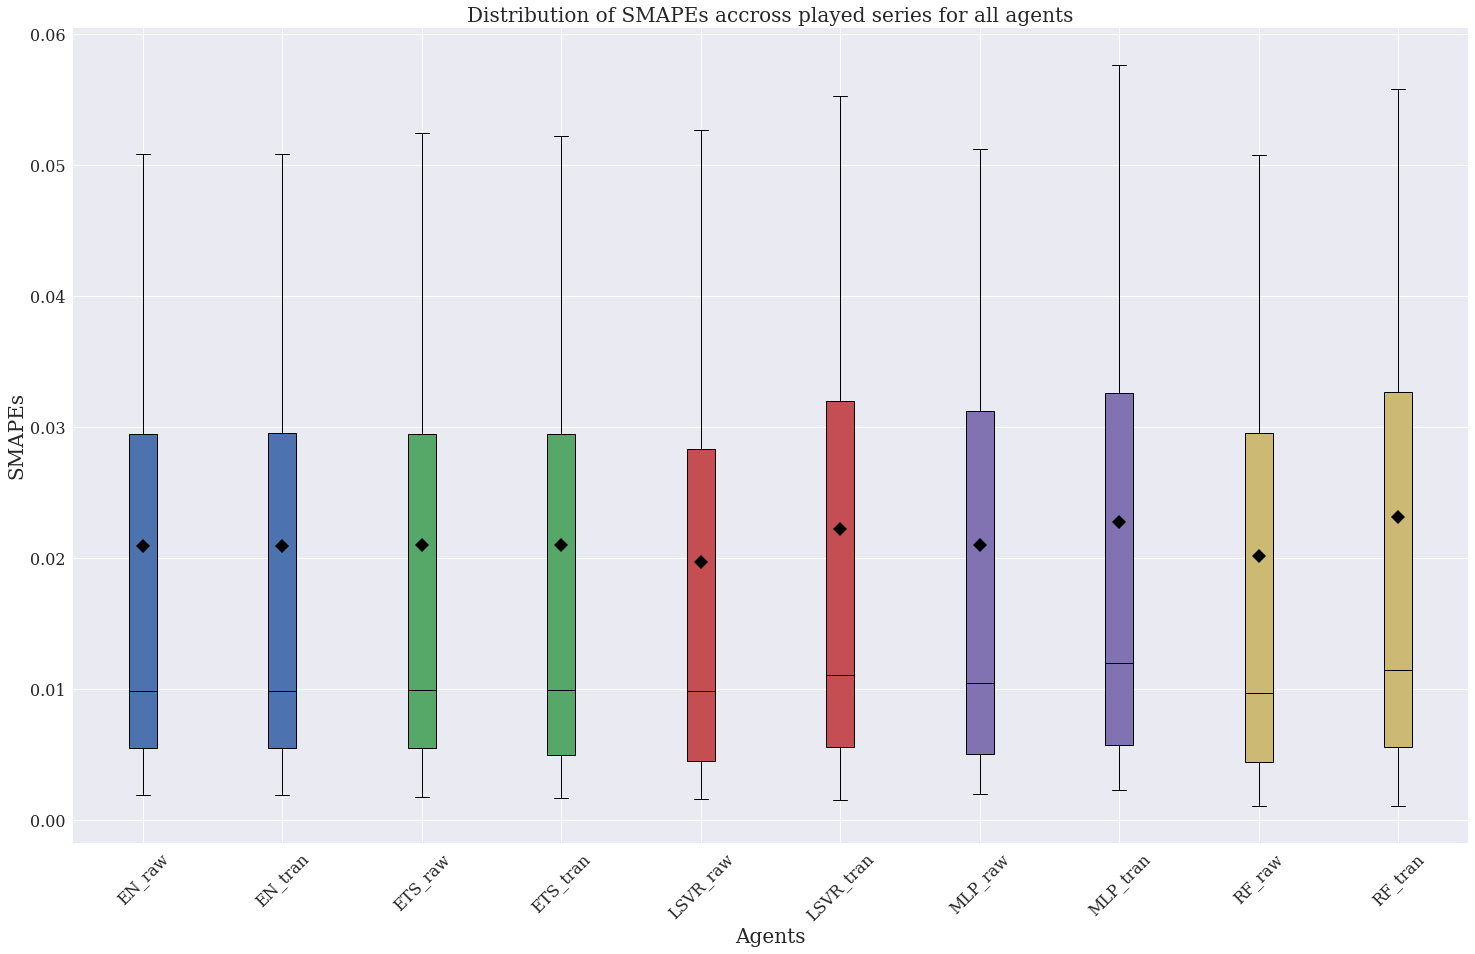
\includegraphics[width=\columnwidth]{weekly_smape_box}
    \caption{Distribution of SMAPE across $66$ weekly time series per agent}
    {\raggedright \footnotesize The dataset used for this graph consists of $66$ weekly financial time series. The boxplots are distributions of SMAPEs (described in Equation \ref{eq: smape}) across $66$ time series per agent. The dimons are the mean of the corresponding distribution. Agents with the same model are colored the same. \par}
    \label{fig: weekly smape box}
\end{figure}
Figure \ref{fig: weekly rank interval} shows each agent's 90\% rank interval as prsented in Equation \ref{eq: rank interval}. Such statistics has the nature of distinguishing the agents even more because the ranks do not overlap regardless how close the agents's errors are. We can see that linear models like elastic net and exponential smoothing are on the same level of performance with and without DCT compared to the other models.
\begin{figure}[H]
    \centering
    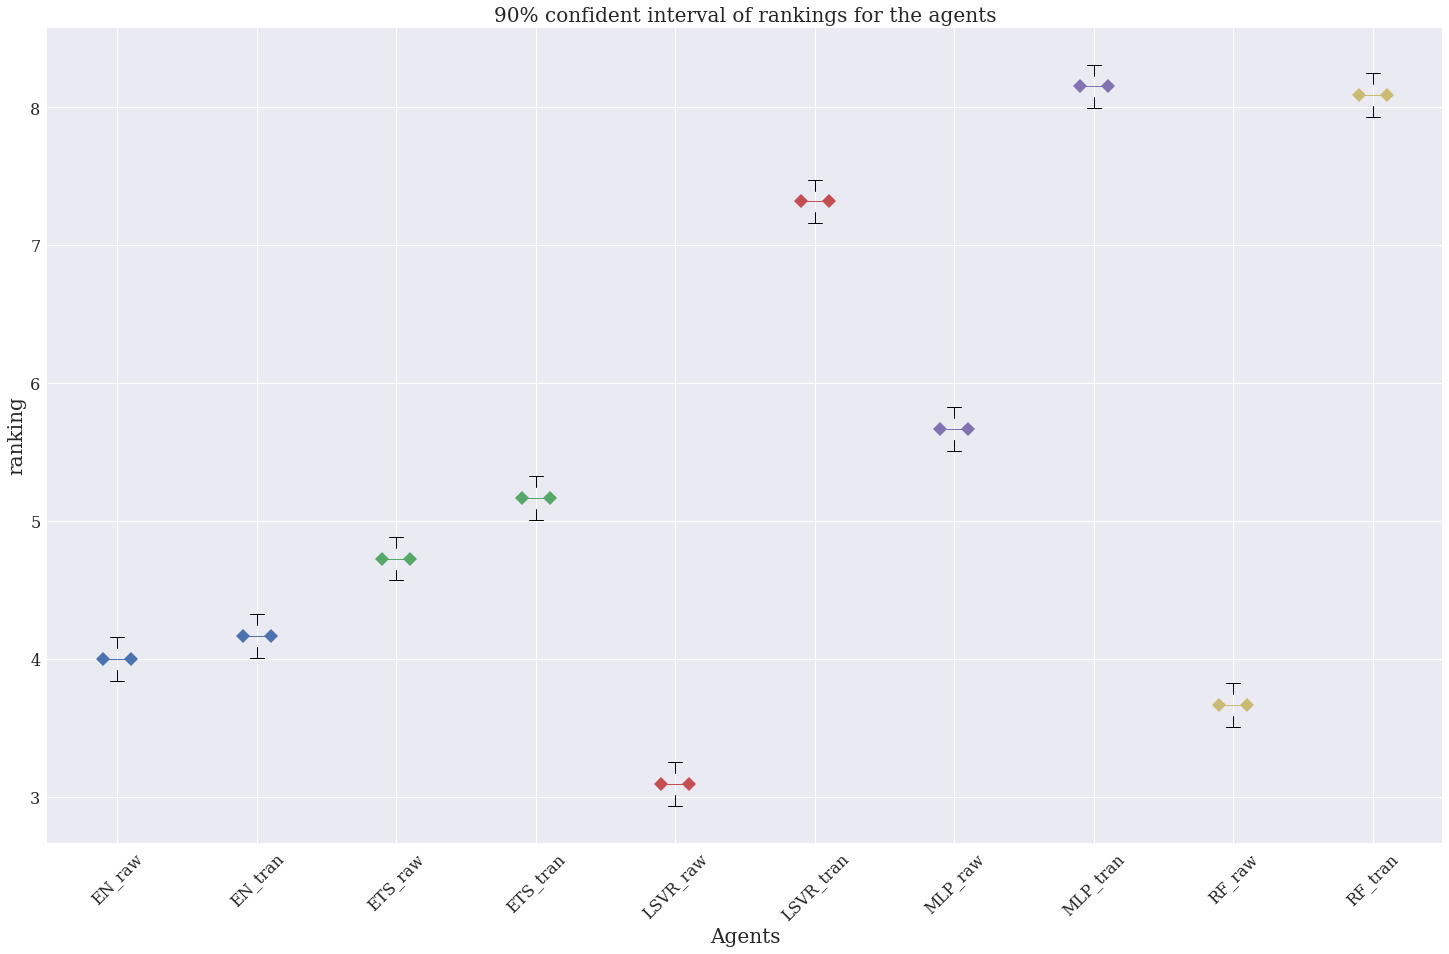
\includegraphics[width=\columnwidth]{weekly_rank_interval}
    \caption{90\% rank interval across $66$ weekly time series per agent}
    {\raggedright \footnotesize The dataset used for this graph consists of $66$ weekly financial time series. The intervals are rank intervals under 90\% confidence level (Equation \ref{eq: rank interval}) over $66$ time series per agent. Agents with the same model are colored the same. \par}
    \label{fig: weekly rank interval}
\end{figure}
Table \ref{tbl: weekly stats} contains the summary statistics across all agents. The fraction-best score confirms what has been shown in Figure \ref{fig: weekly rank interval} that LSVR\_raw and RF\_raw are the most performant agents and EN and ETS agents generate similar errors with and without DCT.
\begin{table}[H]
    \resizebox{\columnwidth}{!}{\begin{tabular}{|l|r r r r r r|}
        \hline
        {} & Avg. SMAPE & Std. SMAPE & Avg. rank & Std. rank & 90\% rank interval & frac best \\
        \hline\hline
        EN\_raw    &    0.02091 &   0.024271 &          4.0 &        1.954 &            (3.753, 4.247) &     0.121 \\
        EN\_tran   &   0.020935 &   0.024349 &        4.167 &        1.919 &             (3.92, 4.414) &     0.106 \\
        \hline
        ETS\_raw   &   0.020979 &   0.024556 &        4.727 &        2.042 &             (4.48, 4.974) &     0.061 \\
        ETS\_tran  &   0.021029 &    0.02474 &        5.167 &        2.086 &             (4.92, 5.414) &      0.03 \\
        \hline
        LSVR\_raw  &   0.019724 &   0.022382 &        3.091 &        2.227 &            (2.844, 3.338) &     0.348 \\
        LSVR\_tran &   0.022205 &   0.024924 &        7.318 &         2.14 &            (7.071, 7.565) &     0.015 \\
        \hline
        MLP\_raw   &   0.021029 &   0.023338 &        5.667 &        2.749 &             (5.42, 5.914) &      0.03 \\
        MLP\_tran  &   0.022734 &   0.024506 &        8.152 &        2.251 &            (7.905, 8.399) &       0.0 \\
        \hline
        RF\_raw    &   0.020129 &   0.022872 &        3.667 &        2.809 &             (3.42, 3.914) &     0.348 \\
        RF\_tran   &    0.02314 &   0.026118 &        8.091 &        2.598 &            (7.844, 8.338) &     0.045 \\
        \hline
    \end{tabular}}
    \caption{Summary statistics of all agents on weekly financial time series}
    {\raggedright \footnotesize The dataset consists of $66$ time series. Average length of the time series is $1260.70$. The first and second columns are the mean and standard deviation of the SMAPEs for each agent. The third and fourth columns are the mean and standard deviation of the ranks (Equation \ref{eq: rank}) for each agent. The fifth column has the 90\% rank intervals. The final column has the fraction best (Equation \ref{eq: frac best}). \par}
    \label{tbl: weekly stats}
\end{table}

As part of the modelling procedure, target transformation techniques are policies that modeller might consider applying depending on the situation, e.g., the dataset, modelling objective, model constraints and assumptions. It would be too ambitious to harbour the intention of seeing a target transformation technique improves performance for all combinations of models and datasets. The overall statistics we showed is a sanity check about whether using DCT risks worsening model performance in general, and the statistics showed it does not. We then move on to examine how often does DCT work in the favor of model performance and when does it happen. For a model M and $66$ time series, we can compute the $66$ SMAPE reductions caused by DCT. Let $SMAPE_{\text{M\_raw}, i}$ and $SMAPE_{\text{M\_tran}, i}$ be the SMAPE for agent using model M without DCT on time series number $i \in \{1, 2, \cdots, 66\}$ and that with DCT on the same time series $i$. Then the SMAPE reduction caused by DCT for time series $i$ is given by
\begin{equation*}
    \frac{SMAPE_{\text{M\_raw}, i} - SMAPE_{\text{M\_tran}, i}}{SMAPE_{\text{M\_raw}, i}} \times 100 \%.
\end{equation*}
The first and second columns in Table \ref{tbl: weekly smape reduction} contain the mean and standard deviation of SMAPE reductions over $66$ time series per agent. Note that positive reduction means DCT works in the model's favor while negative reduction means it's better not to apply DCT. The third column in Table \ref{tbl: weekly smape reduction} shows the proportion of SMAPE reduction being postive over $66$ time series. And the fourth and fifth columns contain the mean and standard deviation of the positive SMAPE reductions per agent. We can see that although EN and ETS have higher positive SMAPE reduction ratio, their reduction is not significant. And this is not surprising from what we saw in the previous summary statistics. On the other hand, LSVR, MLP and RF have about ten percent of positive SMAPE reduction ratio while the average reduction in these cases are all over ten percent ($11.03\%$ for LSVR, $10.03\%$ for MLP and $16.64\%$ for RF). This is to say that there is a ten percent chance that a modeller should consider using DCT because it reduces SMAPE by at least ten percent on average (see Figure \ref{fig: weekly positive smape reduce box} shows the distribution of positive SMAPE reduction per model).
\begin{table}[H]
    \resizebox{\columnwidth}{!}{\begin{tabular}{|l|r r r r r|}
        \hline
        {} & Avg. \% reduction & Std. \% reduction & + reduction ratio & Avg. + \% reduction & Std. + \% reduction \\
        \hline\hline
        EN   &           -0.04 &            0.18 &              19.70 &              0.05 &              0.06 \\
        ETS  &            0.64 &            8.32 &              24.24 &              4.67 &             16.09 \\
        LSVR &          -13.43 &           16.83 &              10.61 &             11.03 &             20.43 \\
        MLP  &          -12.28 &           19.25 &              12.12 &             10.03 &              7.67 \\
        RF   &          -16.08 &           18.54 &               9.09 &             16.64 &             25.41 \\
        \hline
    \end{tabular}}
    \caption{Statistics of SMAPE reduction (\%) using DCT (weekly finance)}
    {\raggedright \footnotesize This table shows the statistics of SMAPE reduction (in percentage) using DC Transformation. The dataset used consists of $66$ weekly financial time series. The first two columns are the mean and standard deviation of SMAPE reduction for all $66$ time series. The third column is the ratio of SMAPE reduction being positive out of $66$ time series. The fourth and fifth columns are the mean and standard deviation of positive SMAPE reductions. \par}
    \label{tbl: weekly smape reduction}
\end{table}
\begin{figure}[H]
    \centering
    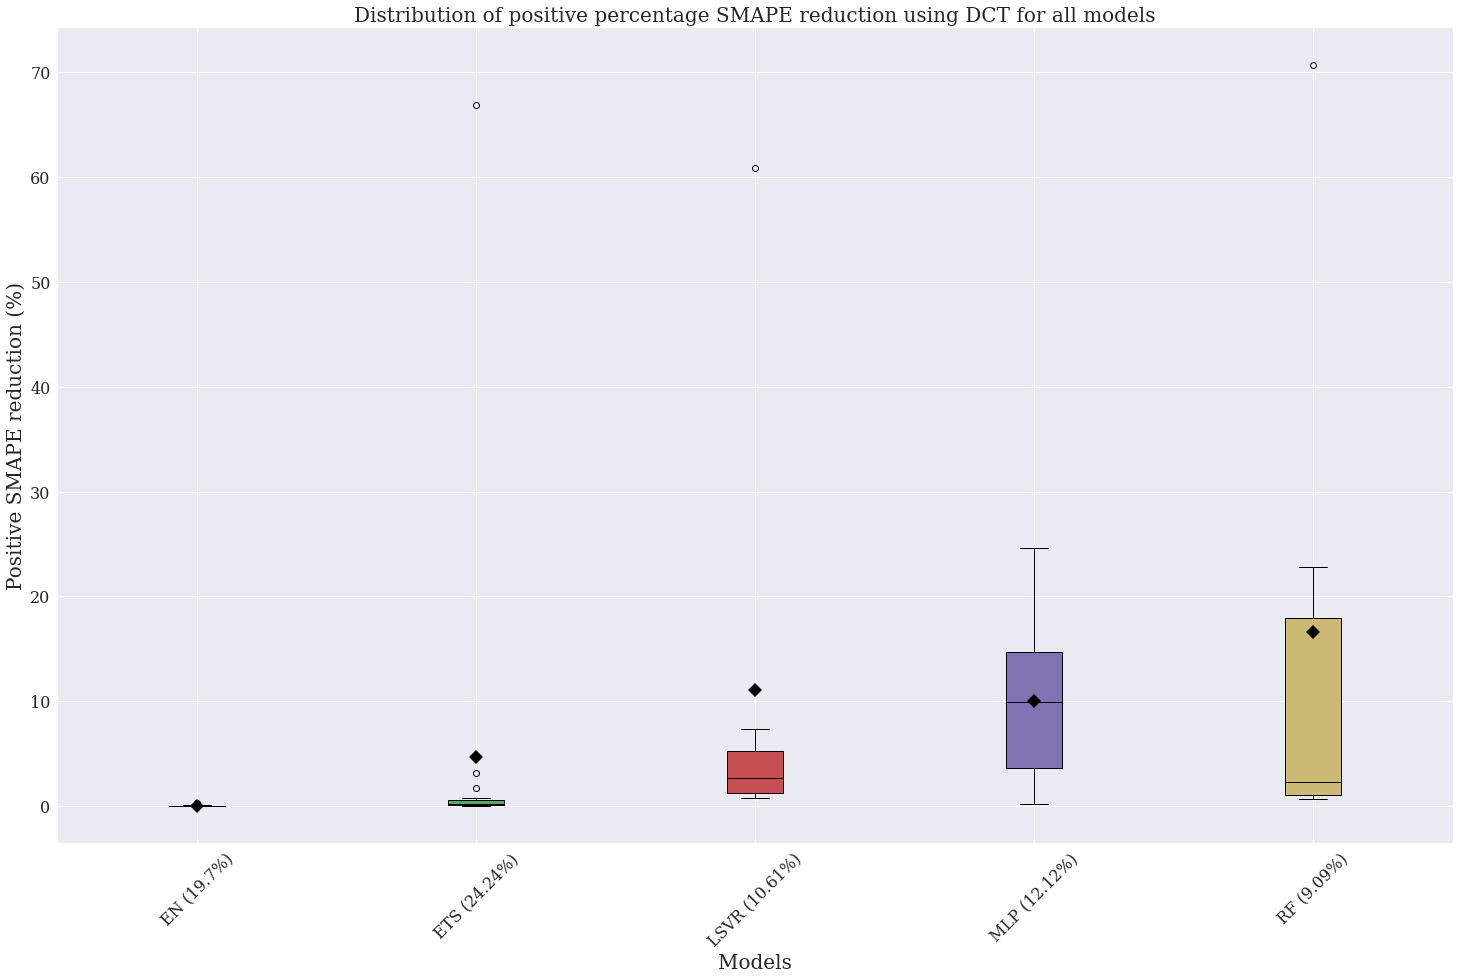
\includegraphics[width=\columnwidth]{weekly_smape_reduce_box_positive}
    \caption{Distribution of positive SMAPE reductions (\%) using DCT}
    {\raggedright \footnotesize The dataset used for this graph consists of $66$ weekly time series in financial domain. The boxplots are the distributions of positive SMAPE reductions (in percentage) using DC Transformation for each models. The dimons are the mean of the corresponding distribution. The number next to the x-labels are the ratio of DCT giving positve SMAPE reductions out of $66$ time series tested.\par}
    \label{fig: weekly positive smape reduce box}
\end{figure}
To investigate how exactly does DCT help reduce SMAPE, we look at some time series of which we have high SMAPE reduction. Figure \ref{fig: weekly 153 ts} is time series number 153 from the M4 dataset. It is a weekly financial time series. Figure \ref{fig: weekly 153 mlp} is MLP's prediction on the test set of time series number 153. The line in blue is the original data. The line in green marks the predictions of MLP without DCT. The line in red marks the predictions of MLP with DCT. On this test, MLP with DCT generates $24.6554\%$ less error compared to MLP without DCT. We can see that the red line follows the blue line better while the green line floats above it. It seems DCT helps MLP to be more responsive to the downward trend.
\begin{figure}[H]
    \centering
    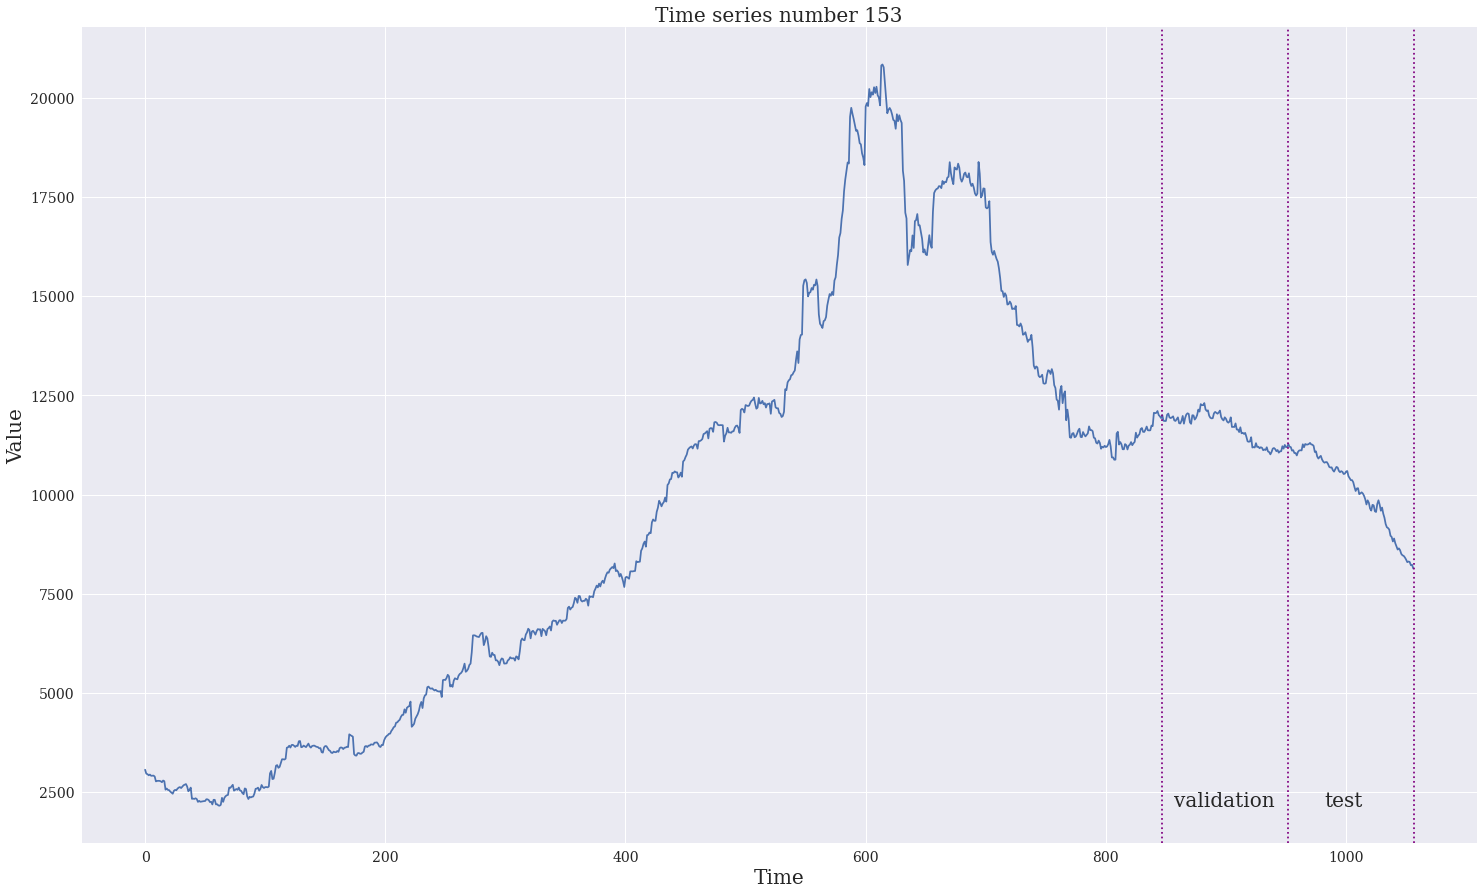
\includegraphics[width=\columnwidth]{weekly_153_ts}
    \caption{Time series No. 153 from M4 dataset}
    {\raggedright \footnotesize Time series No. 153 from M4 dataset is a weekly financial time series. We mark the segments used for validation (model selection) and testing.\par}
    \label{fig: weekly 153 ts}
\end{figure}
\begin{figure}[H]
    \centering
    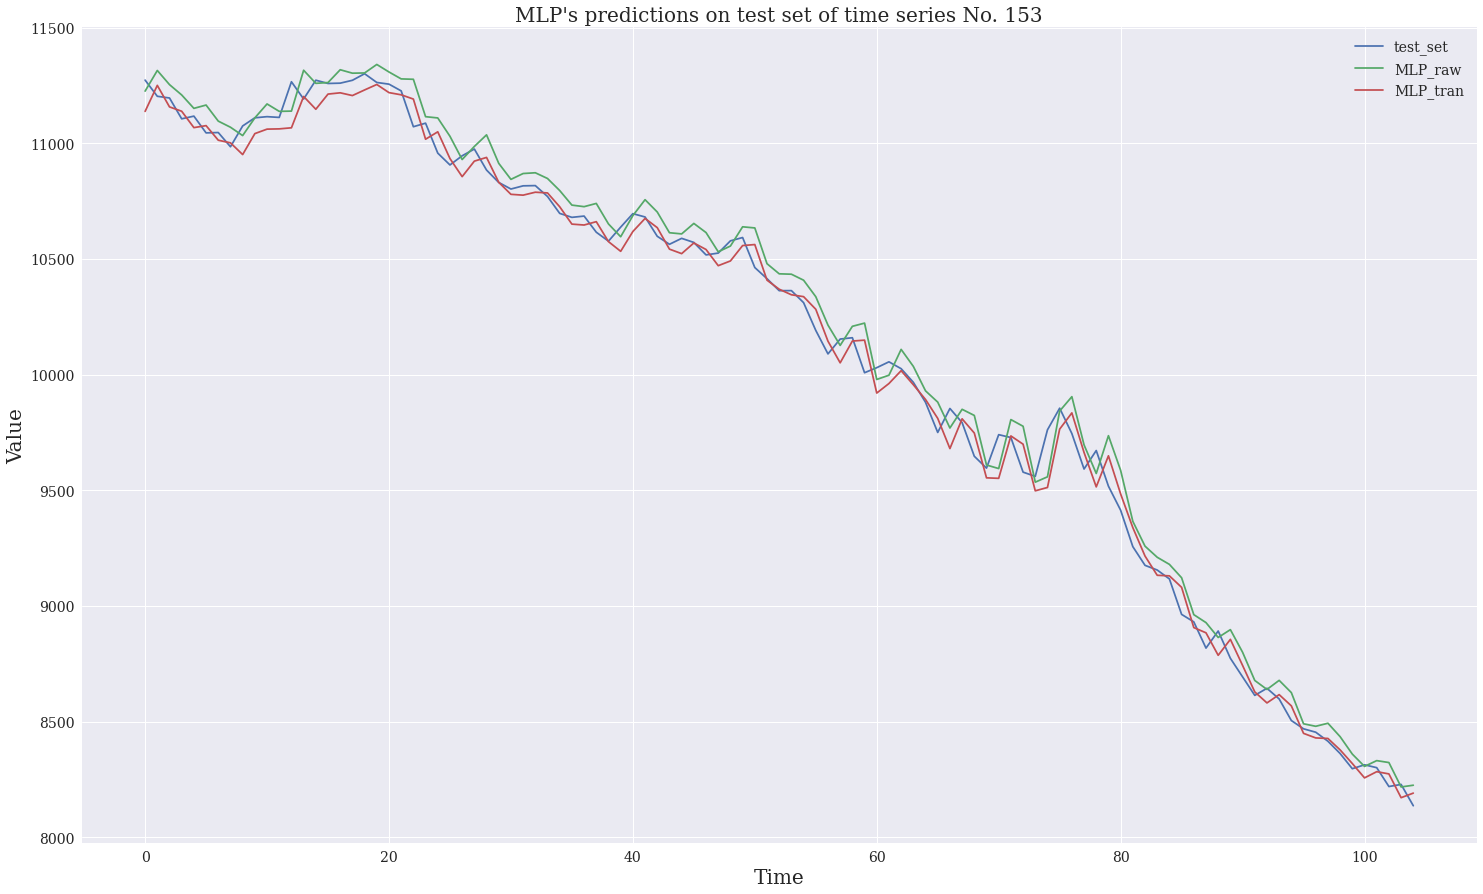
\includegraphics[width=\columnwidth]{weekly_153_mlp}
    \caption{MLP on time series No. 153 from M4 dataset}
    {\raggedright \footnotesize This is MLP's prediction on the test set of time series No. 153 from M4 dataset.  \par}
    \label{fig: weekly 153 mlp}
\end{figure}
Figure \ref{fig: weekly 210 ts} is time series number 210 and Figure \ref{fig: weekly 210 rf} is RF's precition on the test set. We can see that the green line, although corrects itself immediately, tends to deviate away from the blue line even though it shouldn't. We suppose DCT emphases the current trend and stops RF from being impacted by the turbulence observed in the training set.
\begin{figure}[H]
    \centering
    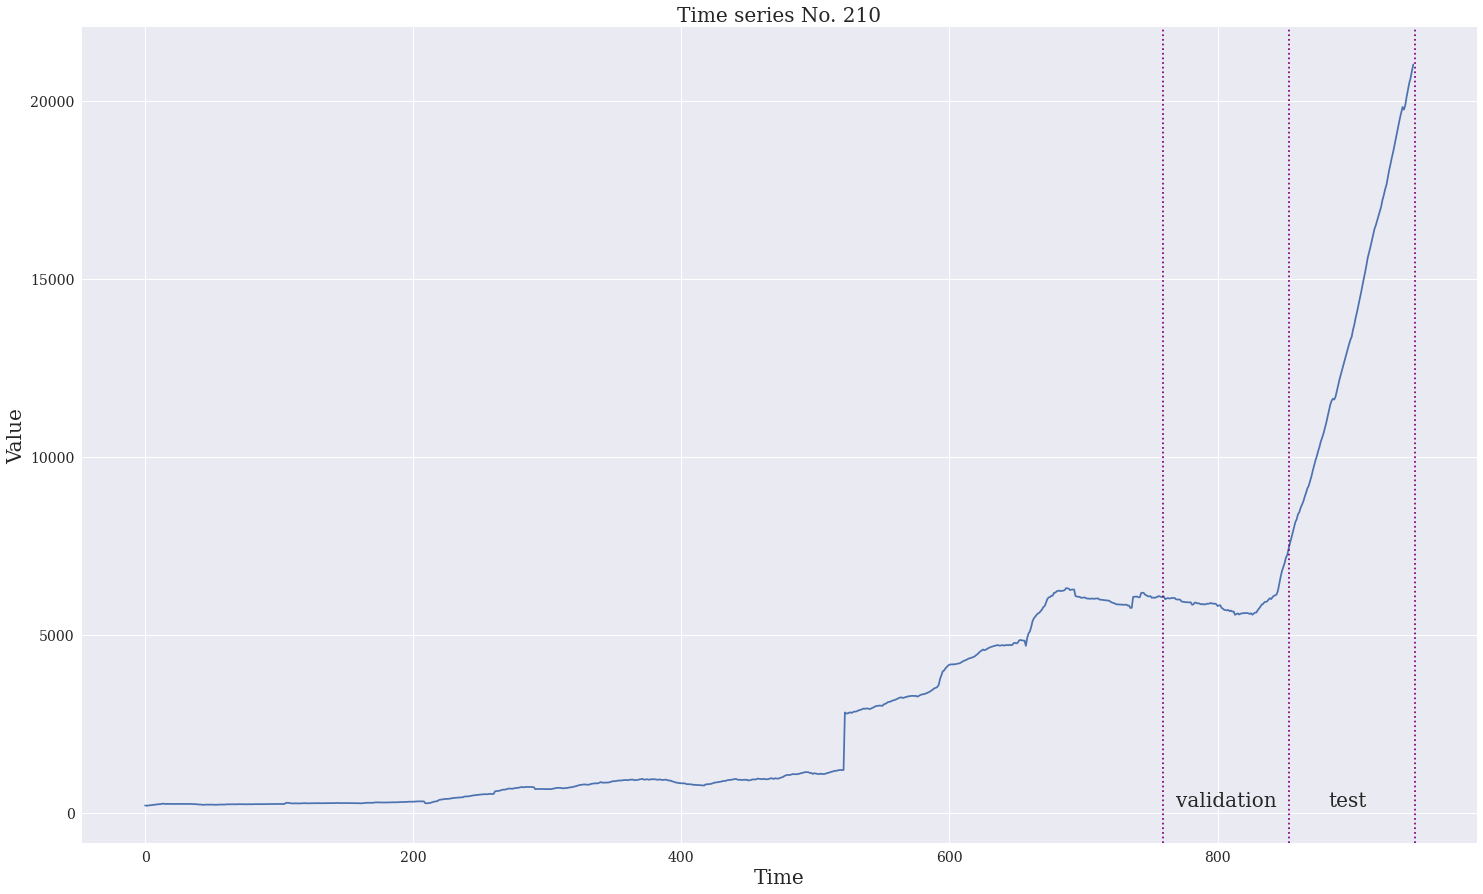
\includegraphics[width=\columnwidth]{weekly_210_ts}
    \caption{Time series No. 210 from M4 dataset}
    {\raggedright \footnotesize Time series No. 210 from M4 dataset is a weekly financial time series. We mark the segments used for validation (model selection) and testing.\par}
    \label{fig: weekly 210 ts}
\end{figure}
\begin{figure}[H]
    \centering
    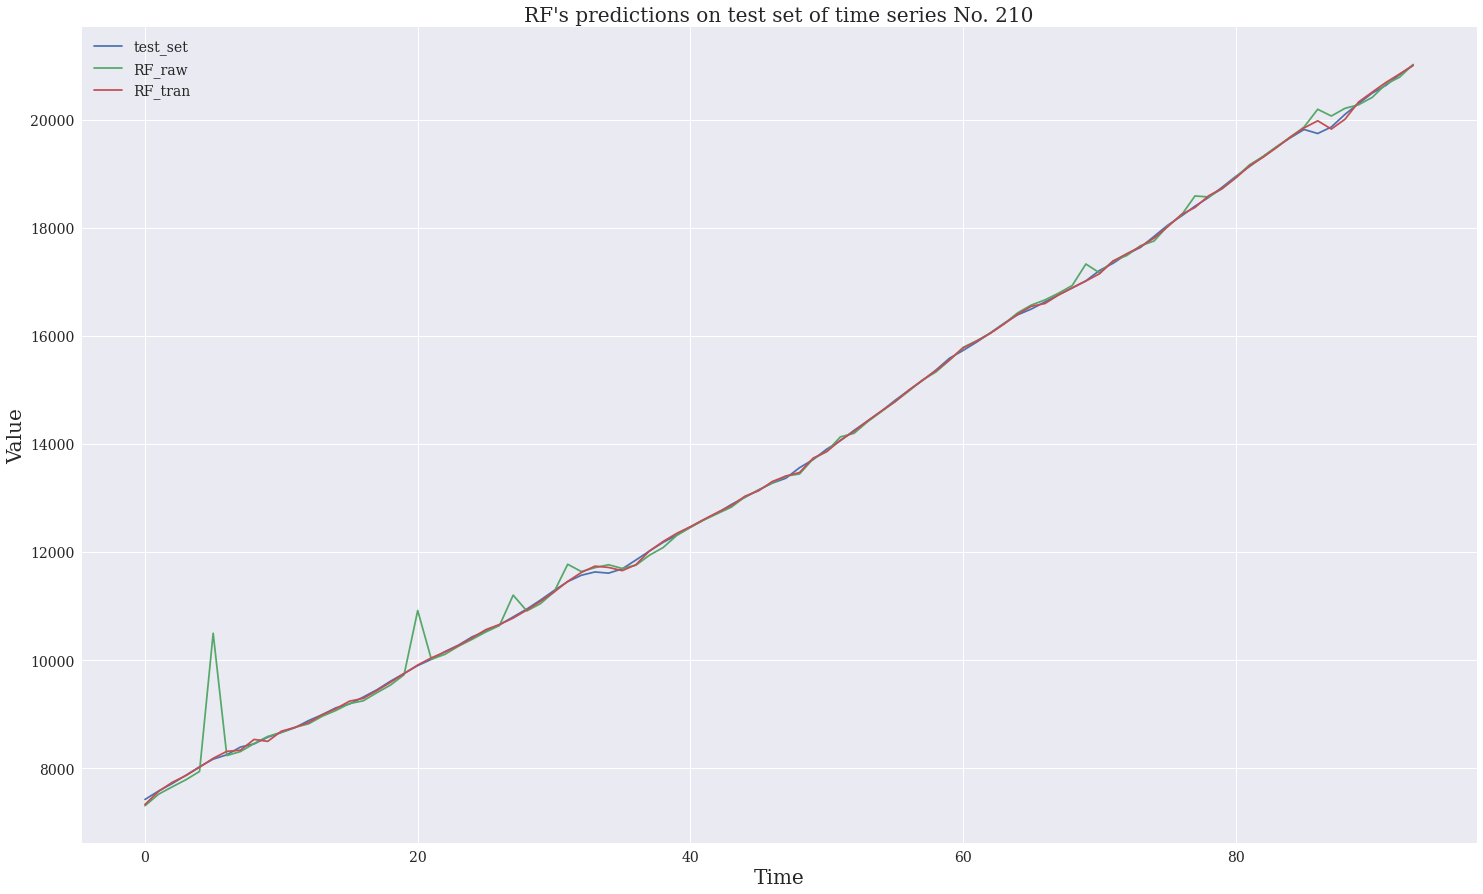
\includegraphics[width=\columnwidth]{weekly_210_rf}
    \caption{RF on time series No. 210 from M4 dataset}
    {\raggedright \footnotesize This is RF's prediction on the test set of time series No. 210 from M4 dataset. The line in blue is the original data. The line in green marks the predictions of RF without DCT. The line in red marks the predictions of RF with DCT. On this test, RF with DCT generates $70.7207\%$ less error compared to RF without DCT. \par}
    \label{fig: weekly 210 rf}
\end{figure}

% \newpage
\section{Analysing Daily Time Series}
As to the daily results in Microeconomics, Macroeconomics and Finance, Figure \ref{fig: daily smape box} shows the distributions of SMAPEs for all $252$ daily time series tested per agent. Figure \ref{fig: daily rank interval} illustrates the agents' respective 90\% confidence interval ranking. And Table \ref{tbl: daily stats} has all the summary statistics. Similar to what has been observed for weekly time series, applying DCT does not impact the overall performance for all models and linear models continue to be top performant compared to others. Given the nature that DC framework is sensitive to frequency of the time series, we estimate that moving from weekly to daily frequency is not significant enough for the algorithm to generate different impact.
\begin{figure}[H]
    \centering
    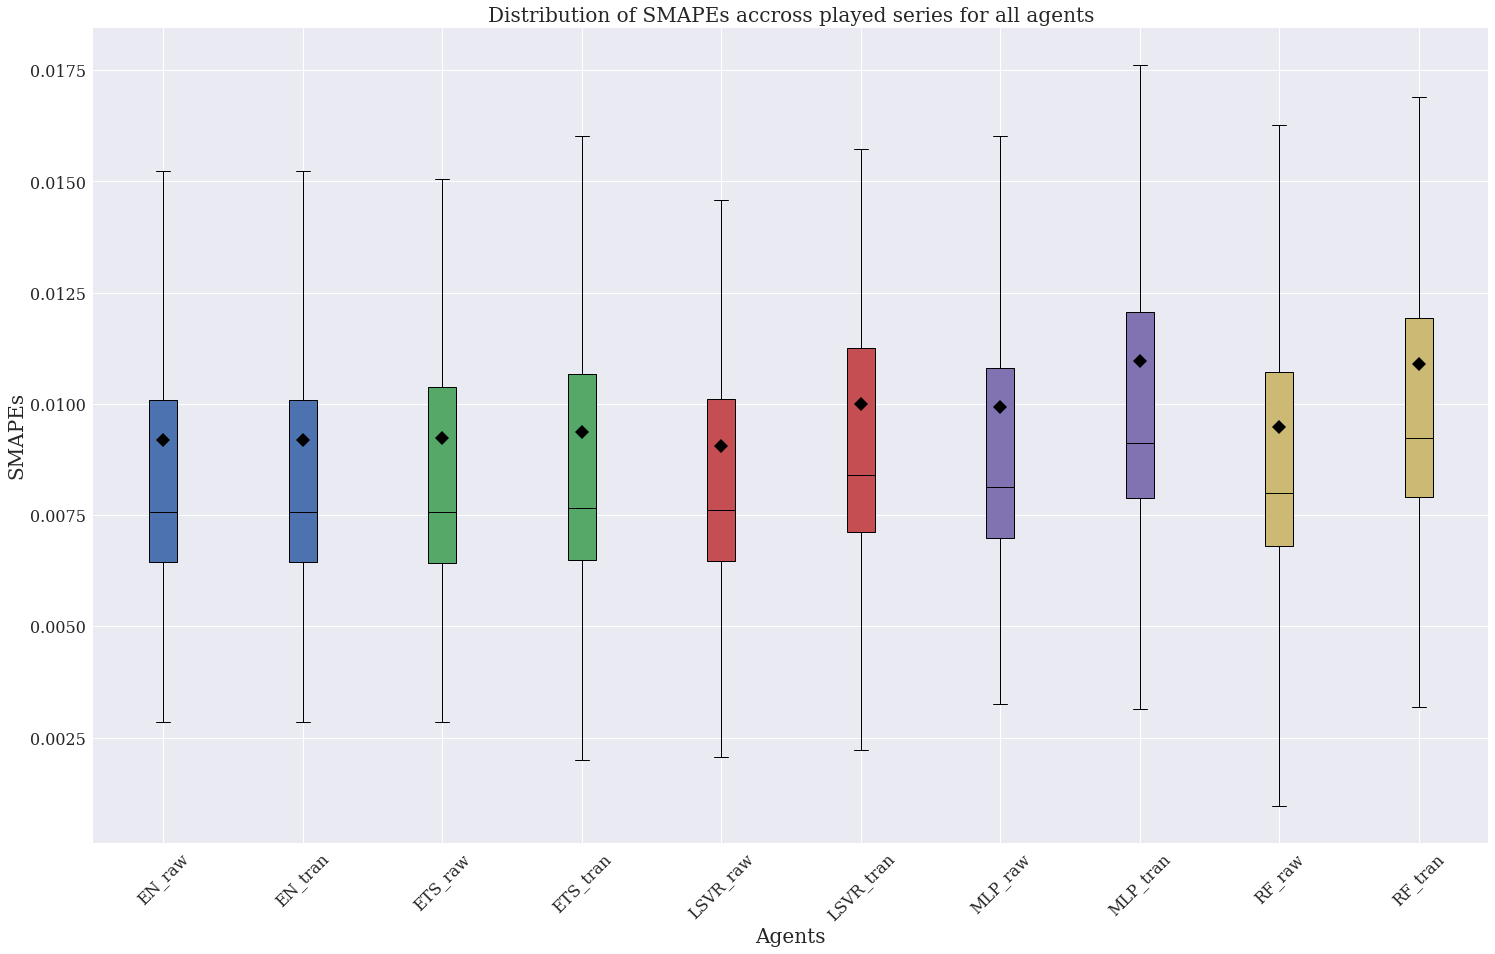
\includegraphics[width=\columnwidth]{daily_smape_box}
    \caption{Distribution of SMAPE across $252$ daily time series per agent}
    {\raggedright \footnotesize The dataset used for this graph consists of $252$ daily time series in micro, macro, and financial domains. The boxplots are distributions of SMAPEs (described in Equation \ref{eq: smape}) across all $252$ time series per agent. The dimons are the mean of the corresponding distribution. Agents with the same model are colored the same. \par}
    \label{fig: daily smape box}
\end{figure}
\begin{figure}[H]
    \centering
    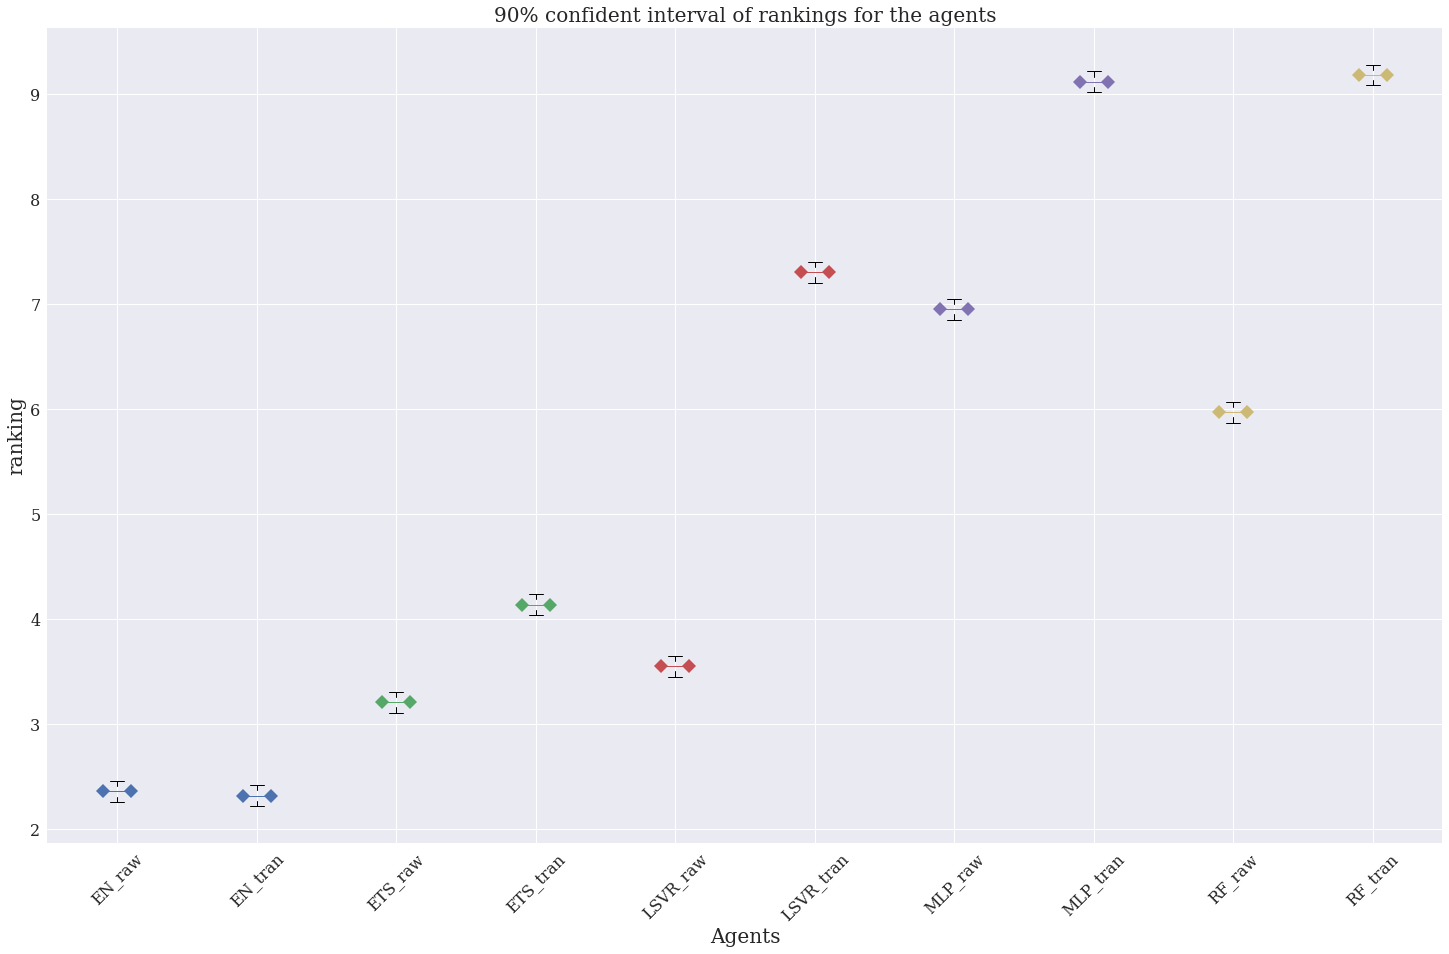
\includegraphics[width=\columnwidth]{daily_rank_interval}
    \caption{90\% rank interval across $252$ daily time series per agent}
    {\raggedright \footnotesize The dataset used for this graph consists of $252$ daily time series. The intervals are rank intervals under 90\% confidence level (Equation \ref{eq: rank interval}) over $252$ time series per agent. Agents with the same model are colored the same. \par}
    \label{fig: daily rank interval}
\end{figure}
\begin{table}[H]
    \resizebox{\columnwidth}{!}{\begin{tabular}{|l|r r r r r r|}
        \hline
        {} & Avg. SMAPE & Std. SMAPE & Avg. rank & Std. rank & 90\% rank interval & frac best \\
        \hline\hline
        EN\_raw    &   0.009179 &    0.00977 &        2.357 &        1.285 &            (2.258, 2.456) &     0.266 \\
        EN\_tran   &   0.009186 &   0.009906 &        2.317 &        1.267 &            (2.218, 2.416) &     0.298 \\
        \hline
        ETS\_raw   &   0.009236 &   0.010134 &        3.206 &         1.57 &            (3.107, 3.305) &     0.175 \\
        ETS\_tran  &   0.009377 &   0.010207 &        4.135 &        1.941 &            (4.036, 4.234) &     0.123 \\
        \hline
        LSVR\_raw  &   0.009059 &   0.007686 &        3.548 &        1.924 &            (3.449, 3.647) &     0.298 \\
        LSVR\_tran &   0.009997 &     0.0107 &        7.302 &        1.326 &            (7.203, 7.401) &     0.004 \\
        \hline
        MLP\_raw   &   0.009934 &   0.008717 &        6.948 &        1.802 &            (6.849, 7.047) &     0.024 \\
        MLP\_tran  &    0.01097 &   0.010123 &        9.115 &        1.109 &            (9.016, 9.214) &       0.0 \\
        \hline
        RF\_raw    &   0.009471 &   0.008224 &        5.968 &        1.898 &            (5.869, 6.067) &     0.075 \\
        RF\_tran   &   0.010889 &   0.010496 &        9.179 &        1.163 &             (9.08, 9.278) &       0.0 \\
        \hline
    \end{tabular}}
    \caption{Summary statistics of all agents on daily time series}
    {\raggedright \footnotesize The dataset consists of $252$ time series including micro, macro and financial domain. Average length of the time series is $1179.99$. The first and second columns are the mean and standard deviation of the SMAPEs for each agent. The third and fourth columns are the mean and standard deviation of the ranks (Equation \ref{eq: rank}) for each agent. The fifth column has the 90\% rank intervals. The final column has the fraction best (Equation \ref{eq: frac best}). \par}
    \label{tbl: daily stats}
\end{table}
Moving on to SMAPE reduction caused by DCT per time series, Table \ref{tbl: daily smape reduction} has the statistics for each model. We can see that linear models continue to have high positive reduction ratio but insignificant reduction. MLP with DCT generates less error $11.51\%$ of the time. Moreover, the mean of these positive reduction is $11.25\%$. Figure \ref{fig: daily positive smape reduce box} has the distributions of positive SMAPE reductions per model.
\begin{table}[H]
    \resizebox{\columnwidth}{!}{\begin{tabular}{|l|r r r r r|}
        \hline
        {} & Avg. \% reduction & Std. \% reduction & + reduction ratio & Avg. + \% reduction & Std. + \% reduction \\
        \hline\hline
        EN   &            0.02 &            0.24 &              23.41 &              0.12 &              0.44 \\
        ETS  &           -1.13 &            3.87 &              30.95 &              0.66 &              3.37 \\
        LSVR &           -9.00 &            5.70 &               3.17 &              1.86 &              1.12 \\
        MLP  &          -12.04 &           17.01 &              11.51 &             11.25 &             10.02 \\
        RF   &          -15.09 &           12.60 &               3.57 &              9.61 &              7.89 \\
        \hline
    \end{tabular}}
    \caption{Statistics of SMAPE reduction (\%) using DCT (daily cross-domain)}
    {\raggedright \footnotesize This table shows the statistics of SMAPE reduction (in percentage) using DC Transformation. The dataset used consists of $252$ daily time series across finance, micro, and macro domains. The first two columns are the mean and standard deviation of SMAPE reduction for all $252$ time series. The third column is the ratio of SMAPE reduction being positive out of $252$ time series. The fourth and fifth columns are the mean and standard deviation of positive SMAPE reductions. \par}
    \label{tbl: daily smape reduction}
\end{table}
\begin{figure}[H]
    \centering
    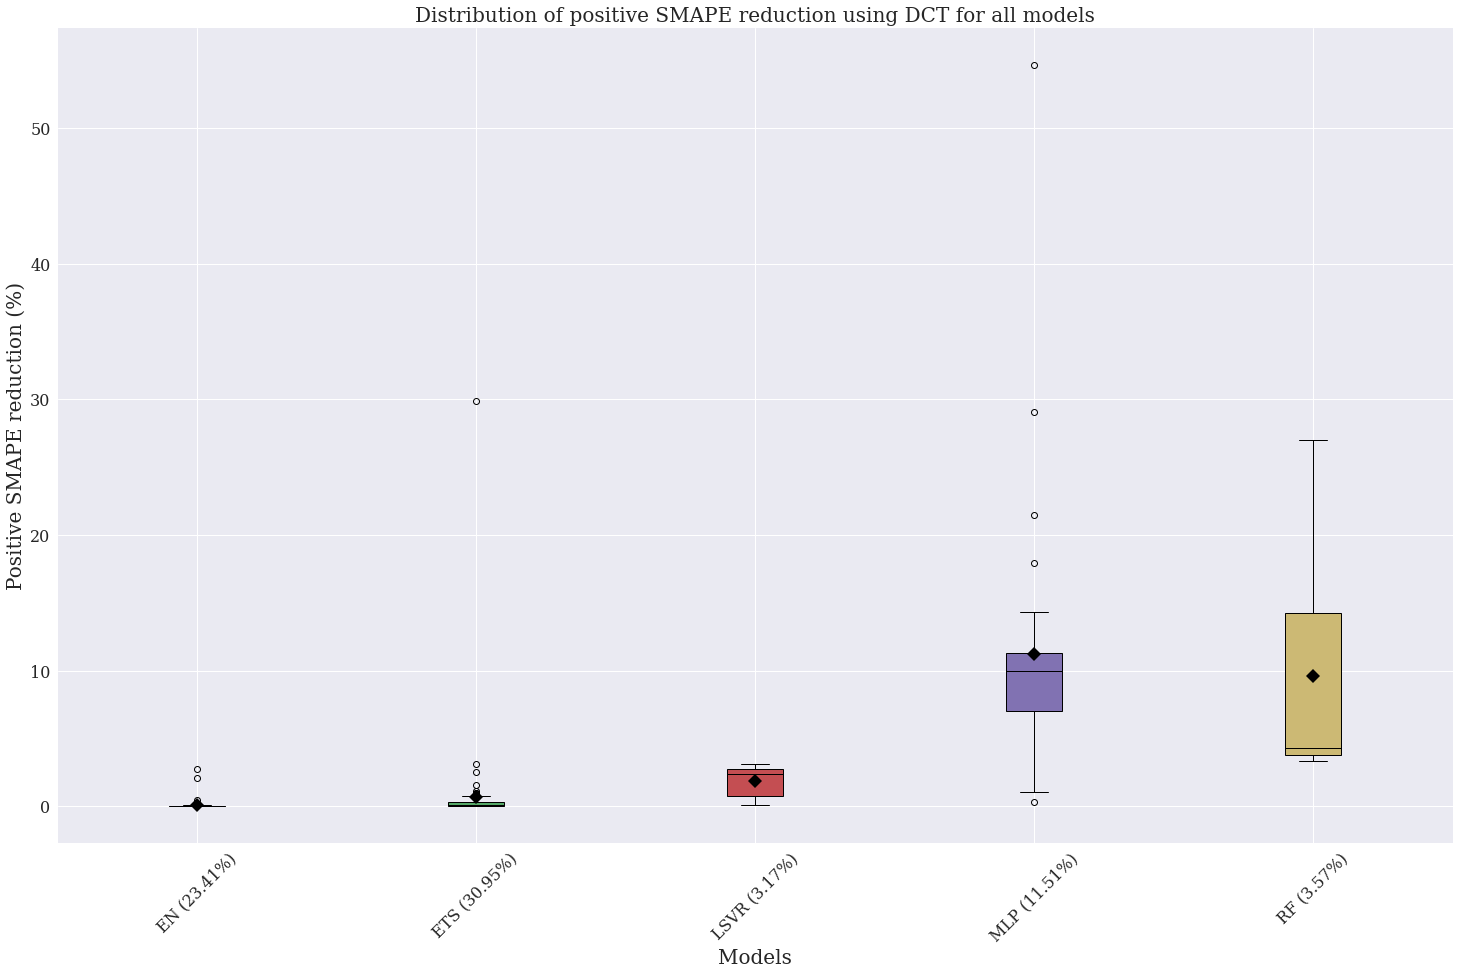
\includegraphics[width=\columnwidth]{daily_smape_reduce_box_positive}
    \caption{Distribution of positive SMAPE reductions (\%) using DCT}
    {\raggedright \footnotesize The dataset used for this graph consists of $252$ daily time series in micro, macro and financial domain. The boxplots are the distributions of positive SMAPE reductions (in percentage) using DC Transformation for each models. The dimons are the mean of the corresponding distribution. The number next to the x-labels are the ratio of DCT giving positve SMAPE reductions out of $252$ time series tested.\par}
    \label{fig: daily positive smape reduce box}
\end{figure}
To look into how the models are doing, Figure \ref{fig: daily 35 ts} is a daily macro time series numbered 35 in M4 dataset and Figure \ref{fig: daily 35 ets} has the predictions generated by ETS in the test set. SMAPE reduction caused by DCT in this figure is $29.8947\%$. We can observe the similar characteristics from what we saw in the weekly time series that agent with DCT reacts faster and more accurate to a clear trend.
\begin{figure}[H]
    \centering
    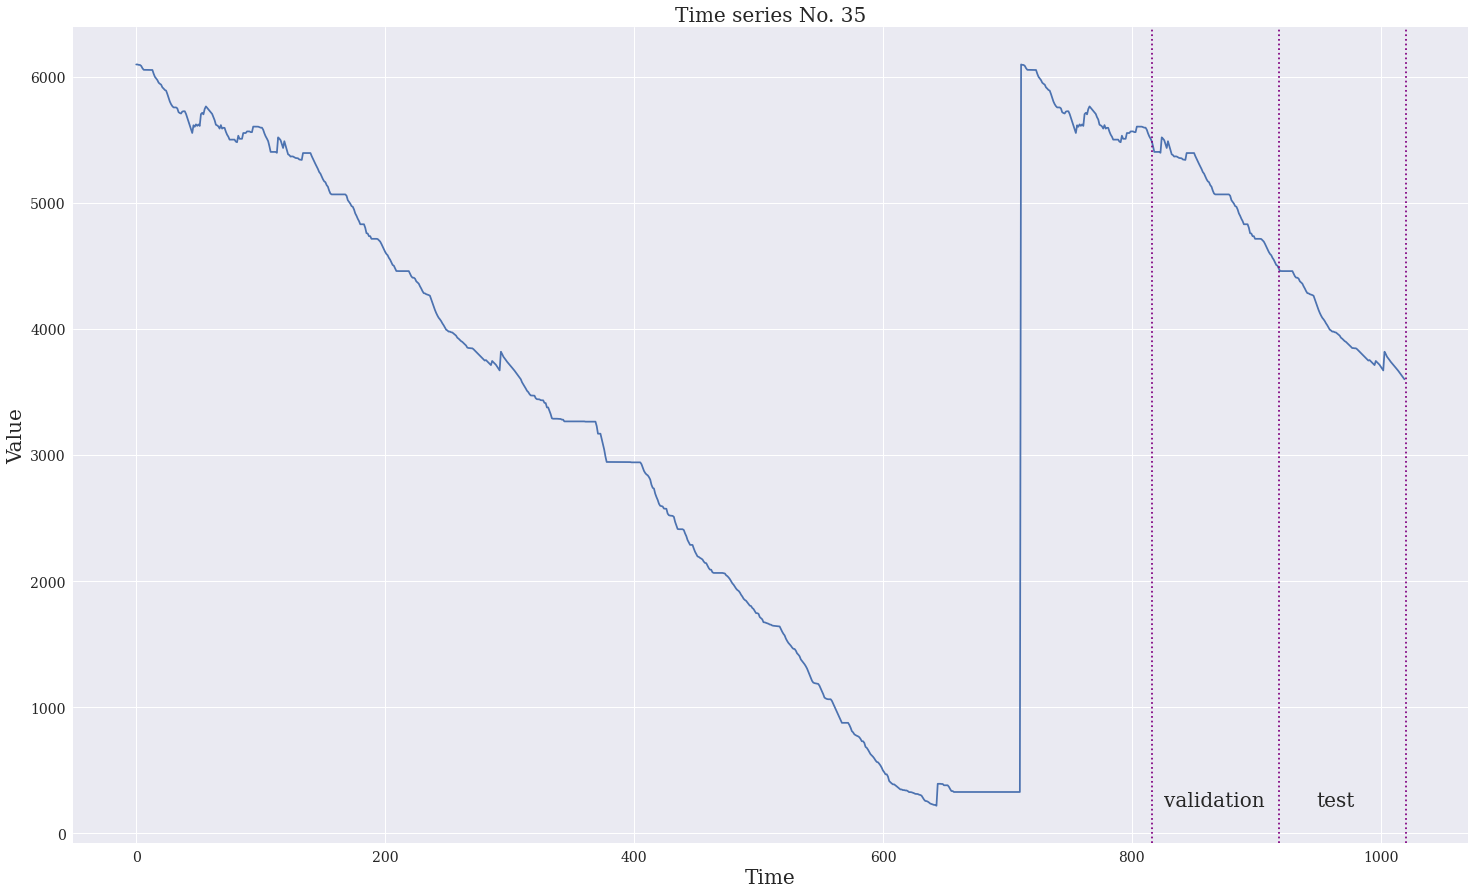
\includegraphics[width=\columnwidth]{daily_35_ts}
    \caption{Time series No. 35 from M4 dataset}
    {\raggedright \footnotesize Time series No. 35 from M4 dataset is a daily macro time series. We mark the segments used for validation (model selection) and testing.\par}
    \label{fig: daily 35 ts}
\end{figure}
\begin{figure}[H]
    \centering
    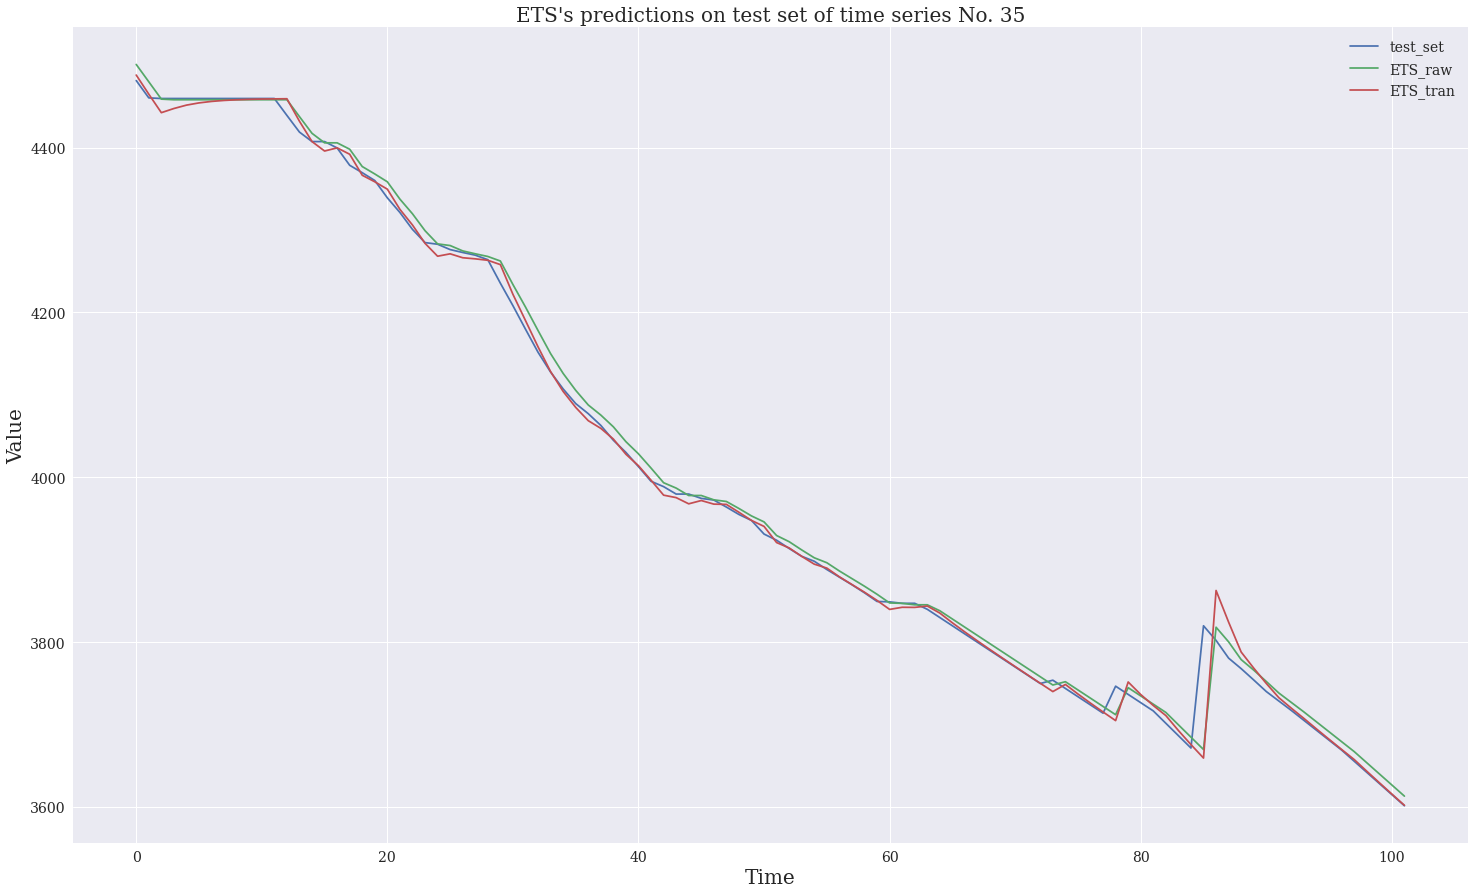
\includegraphics[width=\columnwidth]{daily_35_ets}
    \caption{ETS on time series No. 35 from M4 dataset}
    {\raggedright \footnotesize This is ETS's prediction on the test set of time series No. 35 from M4 dataset.  \par}
    \label{fig: daily 35 ets}
\end{figure}
Figure \ref{fig: daily 69 mlp} is another daily macro time series in M4 dataset and Figure \ref{fig: daily 69 mlp} has the predictions generated by MLP in the test set. DCT reduces $54.6662\%$ of SMAPE in this test. It's clear that MLP\_raw is heavily affected by the drastic rise in the test set and takes a while to accustom to that. On the other hand, MLP\_tran is immune to the shock.
\begin{figure}[H]
    \centering
    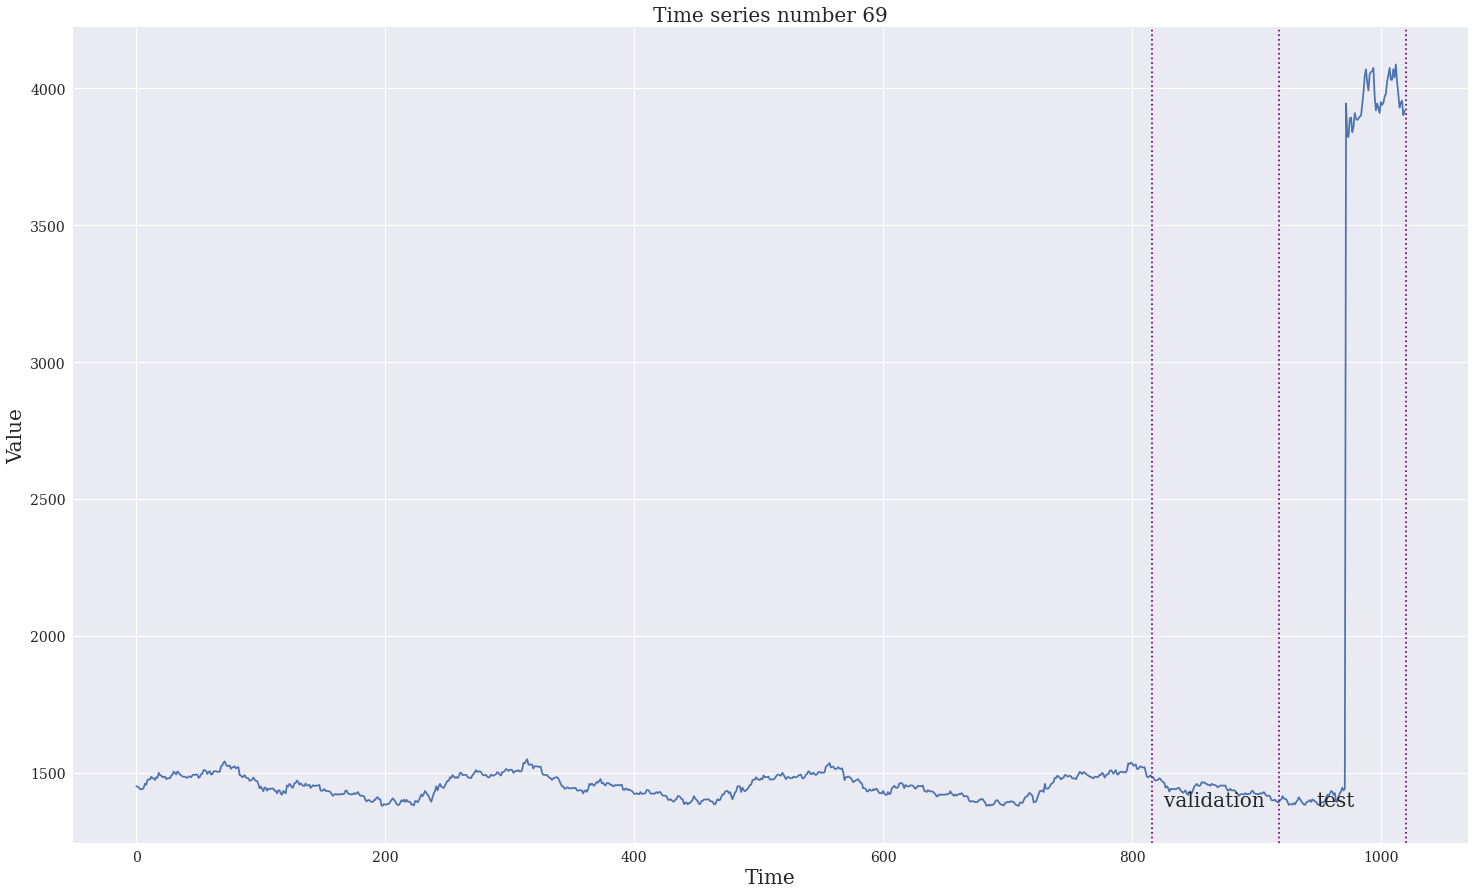
\includegraphics[width=\columnwidth]{daily_69_ts}
    \caption{Time series No. 69 from M4 dataset}
    {\raggedright \footnotesize Time series No. 69 from M4 dataset is a daily macro time series. We mark the segments used for validation (model selection) and testing.\par}
    \label{fig: daily 69 ts}
\end{figure}
\begin{figure}[H]
    \centering
    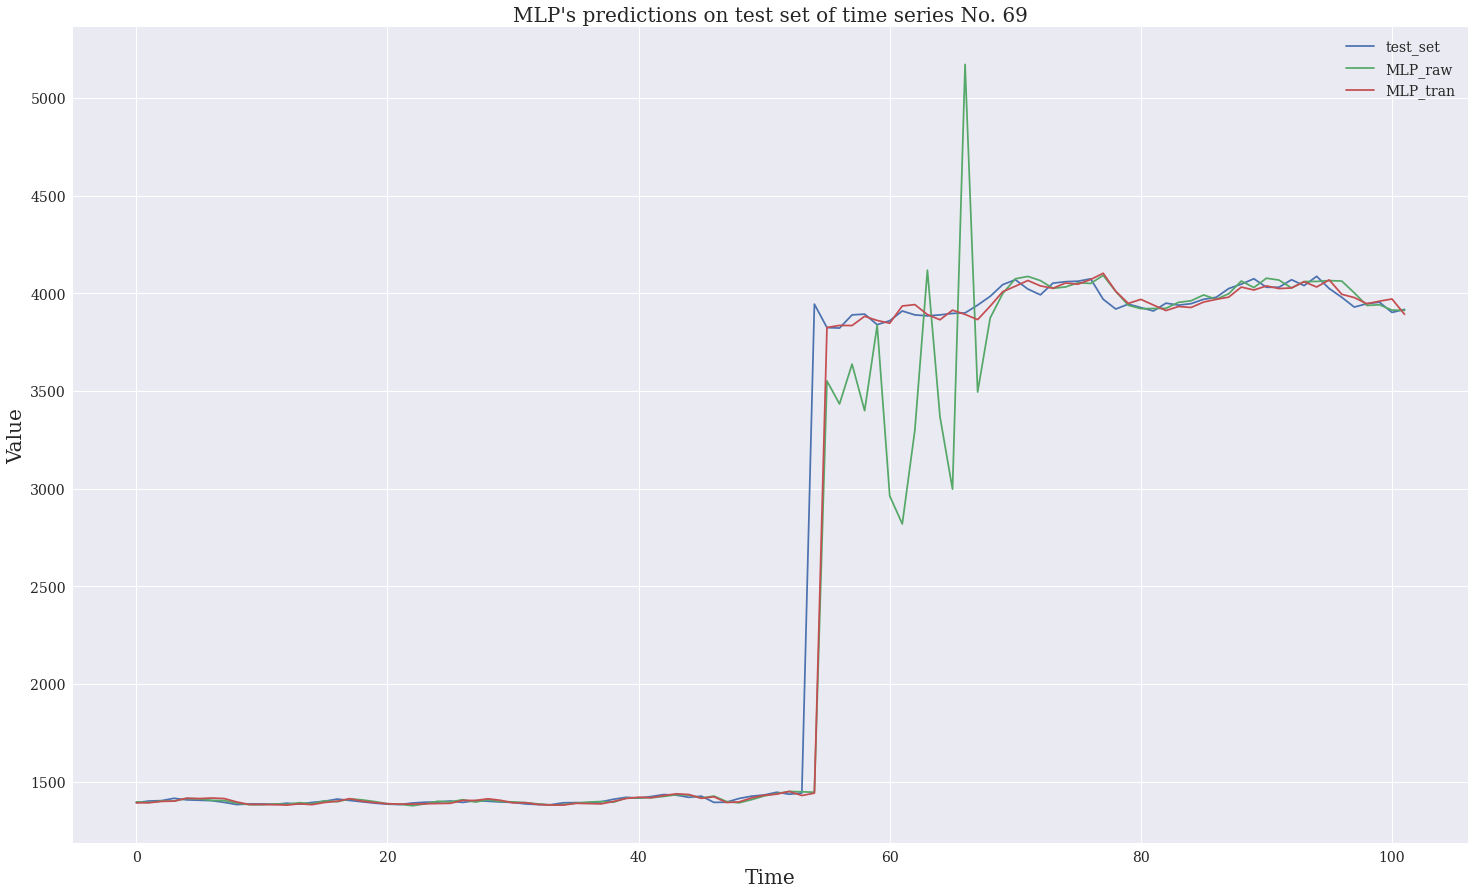
\includegraphics[width=\columnwidth]{daily_69_mlp}
    \caption{MLP on time series No. 69 from M4 dataset}
    {\raggedright \footnotesize This is MLP's prediction on the test set of time series No. 69 from M4 dataset.  \par}
    \label{fig: daily 69 mlp}
\end{figure}

% \newpage
\section{Analysing Hourly Time Series}
We then analyse experimental results concerning 140 hourly time series. Things start to look quite different for hourly time series. Figure \ref{fig: hourly smape box} contains the distributions of SMAPE per agent, Figure \ref{fig: hourly rank interval} has the rank intervals and Table \ref{tbl: hourly stats} holds all the summary statistics. Notice that EN with DCT has significantly smaller error in general.
\begin{figure}[H]
    \centering
    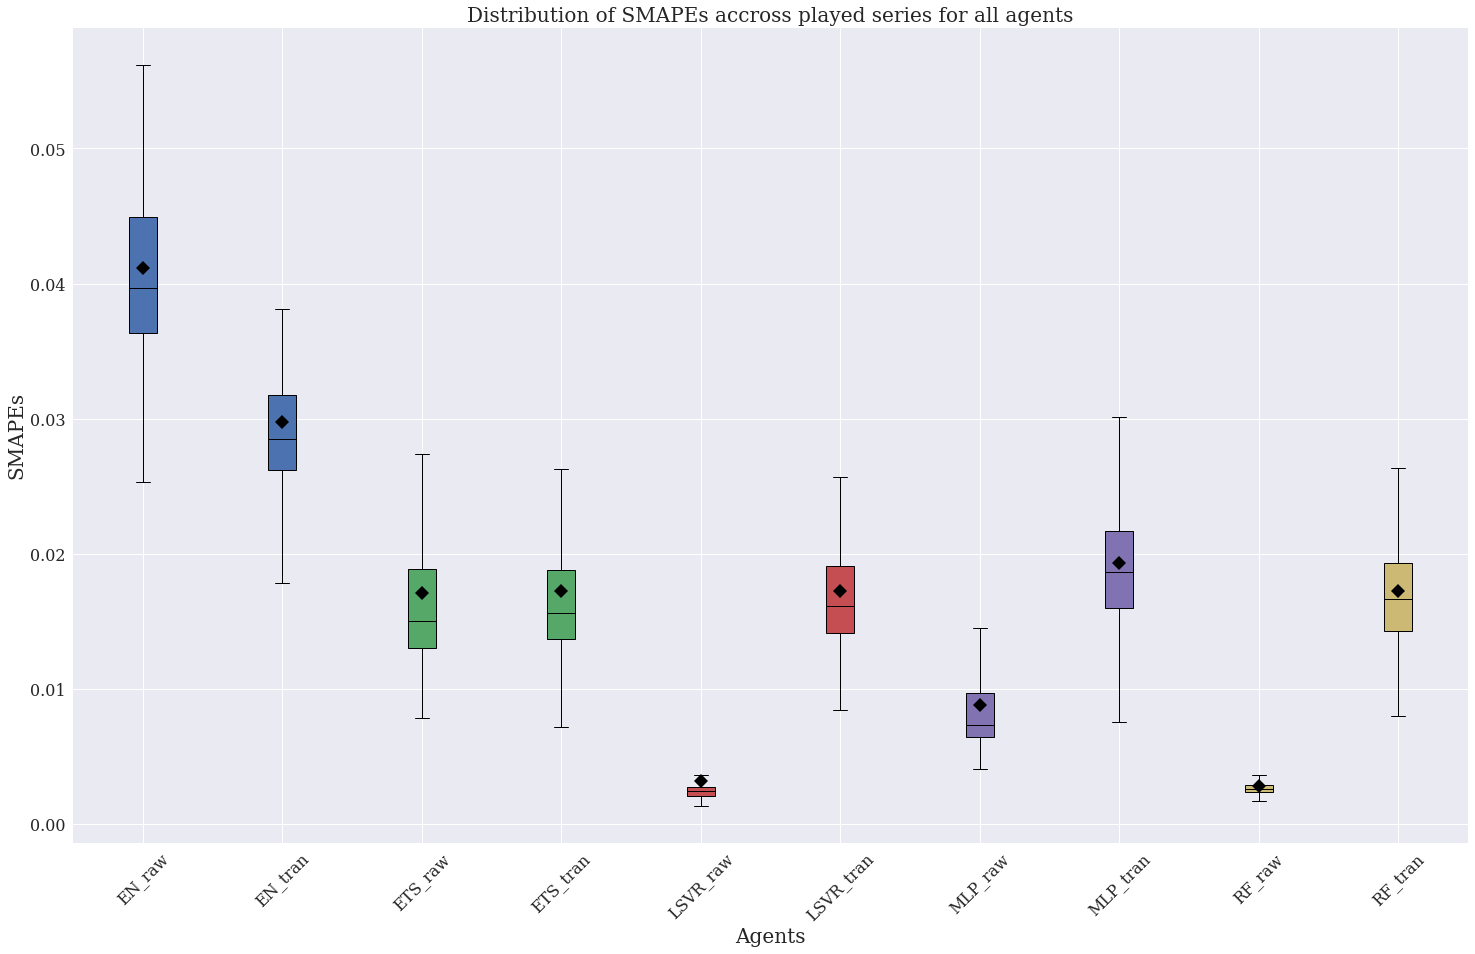
\includegraphics[width=\columnwidth]{hourly_smape_box}
    \caption{Distribution of SMAPE across $140$ hourly time series per agent}
    {\raggedright \footnotesize The dataset used for this graph consists of $140$ hourly time series in unknown domain. The boxplots are distributions of SMAPEs (described in Equation \ref{eq: smape}) across $140$ time series per agent. The dimons are the mean of the corresponding distribution. Agents with the same model are colored the same. \par}
    \label{fig: hourly smape box}
\end{figure}
\begin{figure}[H]
    \centering
    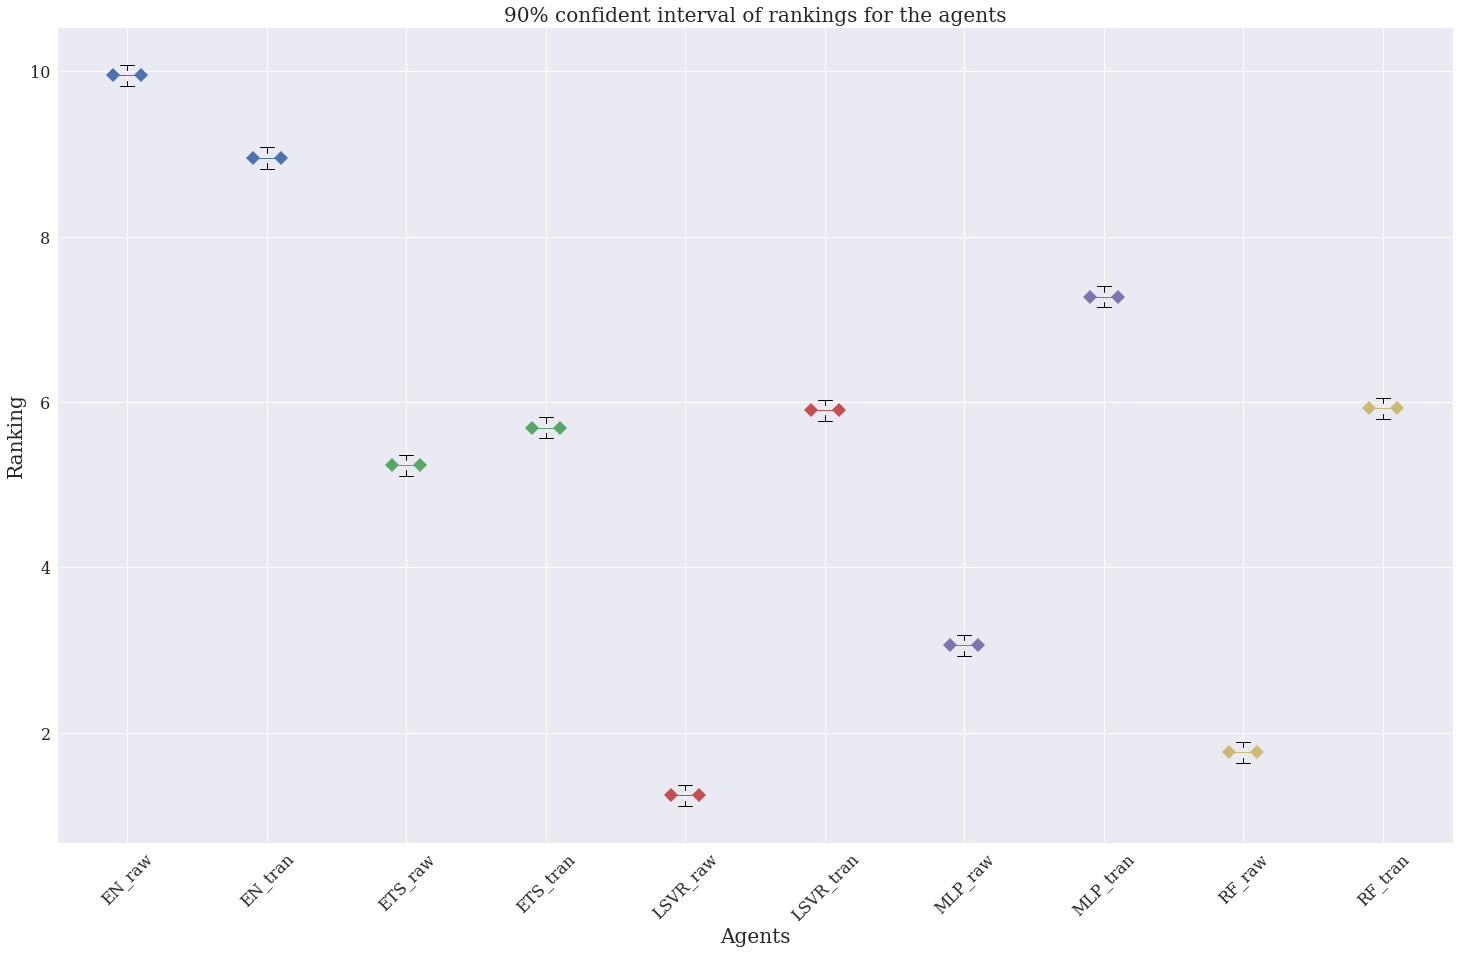
\includegraphics[width=\columnwidth]{hourly_rank_interval}
    \caption{90\% rank interval across $140$ hourly time series per agent}
    {\raggedright \footnotesize The dataset used for this graph consists of $140$ hourly time series. The intervals are rank intervals under 90\% confidence level (Equation \ref{eq: rank interval}) over $140$ time series per agent. Agents with the same model are colored the same. \par}
    \label{fig: hourly rank interval}
\end{figure}
\begin{table}[H]
    \resizebox{\columnwidth}{!}{\begin{tabular}{|l|r r r r r r|}
        \hline
        {} & Avg. SMAPE & Std. SMAPE & Avg. rank & Std. rank & 90\% rank interval & frac best \\
        \hline\hline
        EN\_raw    &   0.041144 &   0.010202 &         9.95 &        0.218 &           (9.822, 10.078) &       0.0 \\
        EN\_tran   &   0.029771 &   0.006564 &         8.95 &        0.525 &            (8.822, 9.078) &       0.0 \\
        \hline
        ETS\_raw   &   0.017082 &   0.007781 &        5.236 &        1.477 &            (5.108, 5.364) &       0.0 \\
        ETS\_tran  &    0.01727 &   0.006678 &        5.686 &        1.063 &            (5.558, 5.814) &       0.0 \\
        \hline
        LSVR\_raw  &   0.003148 &   0.004825 &        1.243 &        0.445 &            (1.115, 1.371) &     0.764 \\
        LSVR\_tran &   0.017249 &   0.005926 &          5.9 &        1.289 &            (5.772, 6.028) &       0.0 \\
        \hline
        MLP\_raw   &   0.008819 &   0.006091 &        3.057 &         0.41 &            (2.929, 3.185) &       0.0 \\
        MLP\_tran  &   0.019317 &   0.006434 &        7.271 &        1.212 &            (7.143, 7.399) &       0.0 \\
        \hline
        RF\_raw    &    0.00284 &   0.002112 &        1.764 &        0.424 &            (1.636, 1.892) &     0.236 \\
        RF\_tran   &   0.017274 &   0.005028 &        5.921 &        1.358 &            (5.793, 6.049) &       0.0 \\
        \hline
    \end{tabular}}
    \caption{Summary statistics of all agents on hourly unknown domain time series}
    {\raggedright \footnotesize The dataset consists of $140$ time series. Average length of the time series is $1008$. The first and second columns are the mean and standard deviation of the SMAPEs for each agent. The third and fourth columns are the mean and standard deviation of the ranks (Equation \ref{eq: rank}) for each agent. The fifth column has the 90\% rank intervals. The final column has the fraction best (Equation \ref{eq: frac best}). \par}
    \label{tbl: hourly stats}
\end{table}

Table \ref{tbl: hourly smape reduction} contains the statistics about SMAPE reductions per time series for the models and Figure \ref{fig: hourly positive smape reduce box} illustrates the distributions of the positive SMAPE reductions. We can see that EN has a 97.14\% positive reduction ratio with the average positive reduction being 27.33\%. Also, LSVR and RF have 0\% positive reduction ratio. Judging from previous summary statistics, we can see the reason being LSVR and RF both do so well without DCT and thus make them really hard to outperform (recall that SMAPE reduction is a relative measure).
\begin{table}[H]
    \resizebox{\columnwidth}{!}{\begin{tabular}{|l|r r r r r|}
        \hline
        {} & Avg. \% reduction & Std. \% reduction & + reduction ratio & Avg. + \% reduction & Std. + \% reduction \\
        \hline\hline
        EN   &           26.55 &            7.72 &              97.14 &             27.33 &              6.33 \\
        ETS  &           -3.09 &            9.02 &              27.86 &              5.75 &             10.30 \\
        LSVR &         -598.10 &          211.77 &               0.00 &               NaN &               NaN \\
        MLP  &         -135.48 &           46.83 &               0.71 &              9.02 &              0.00 \\
        RF   &         -548.46 &          161.49 &               0.00 &               NaN &               NaN \\
        \hline
    \end{tabular}}
    \caption{Statistics of SMAPE reduction (\%) using DCT (hourly unknown domain)}
    {\raggedright \footnotesize This table shows the statistics of SMAPE reduction (in percentage) using DC Transformation. The dataset used consists of $140$ hourly time series in unknown domain. The first two columns are the mean and standard deviation of SMAPE reduction for all $140$ time series. The third column is the ratio of SMAPE reduction being positive out of $140$ time series. The fourth and fifth columns are the mean and standard deviation of positive SMAPE reductions. Due to not having any positive reduction, LSVR and RF have NaN values in the fourth and fifth columns. \par}
    \label{tbl: hourly smape reduction}
\end{table}
\begin{figure}[H]
    \centering
    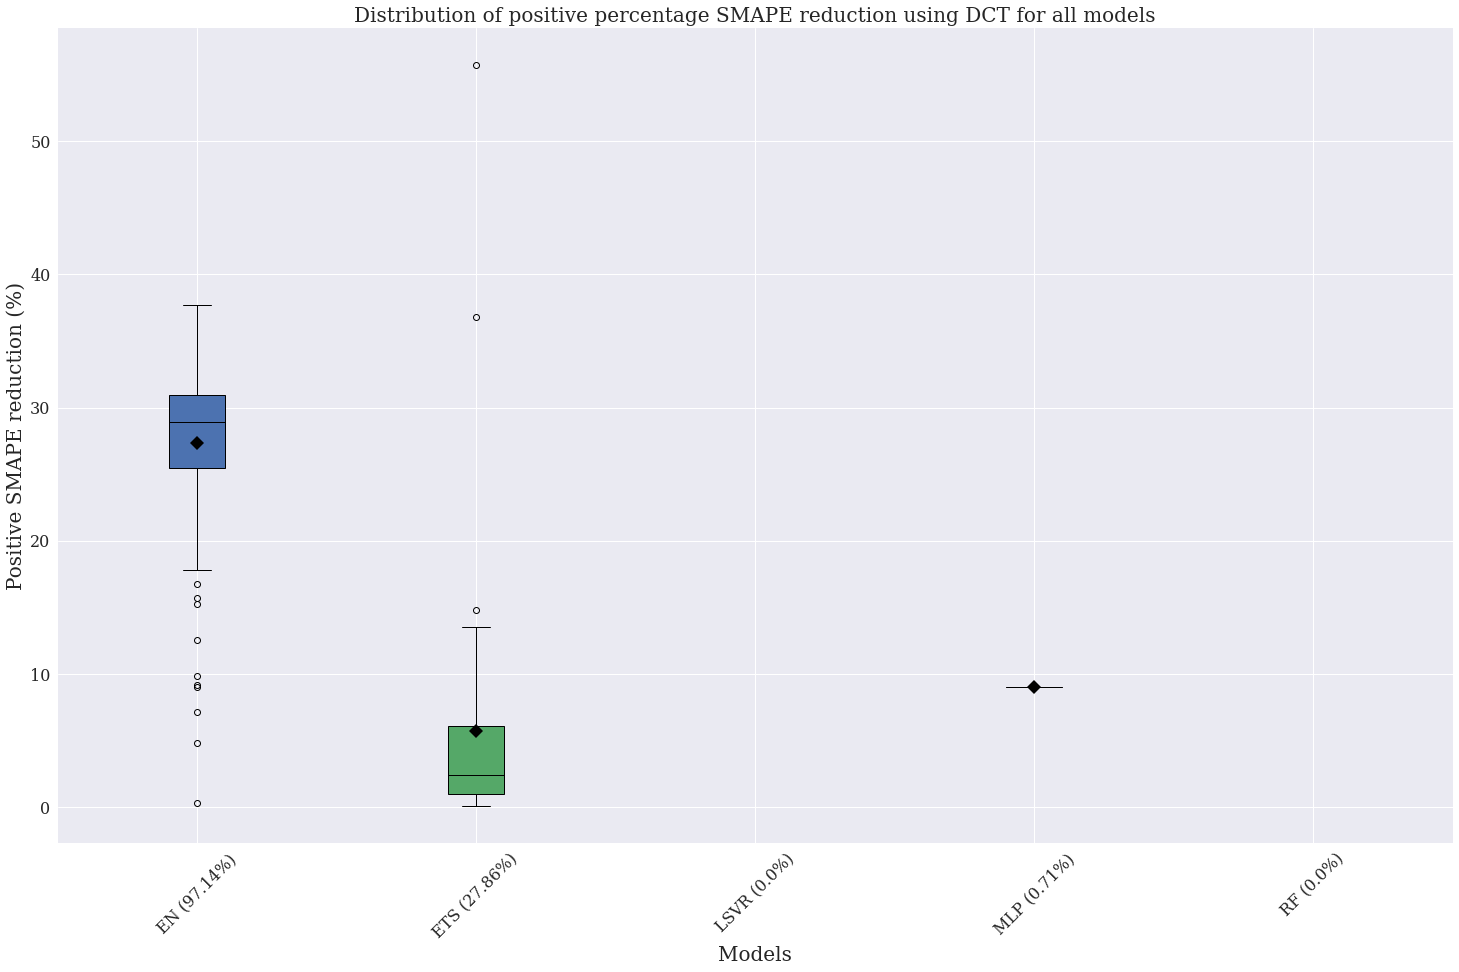
\includegraphics[width=\columnwidth]{hourly_smape_reduce_box_positive}
    \caption{Distribution of positive SMAPE reductions (\%) using DCT}
    {\raggedright \footnotesize The dataset used for this graph consists of $140$ hourly time series in unknown domain. The boxplots are the distributions of positive SMAPE reductions (in percentage) using DC Transformation for each models. The dimons are the mean of the corresponding distribution. The number next to the x-labels are the ratio of DCT giving positve SMAPE reductions out of $140$ time series tested.\par}
    \label{fig: hourly positive smape reduce box}
\end{figure}

To further investigate model behaviours, we look at time series number 271 (see Figure \ref{fig: hourly 271 ts}), which is of hourly frequency but unknown domain. It's clear that such time series has very different behaviours from what we have previously for micro, macro, and financial domain. It turns out most time series of hourly frequency we tested are like this.
\begin{figure}[H]
    \centering
    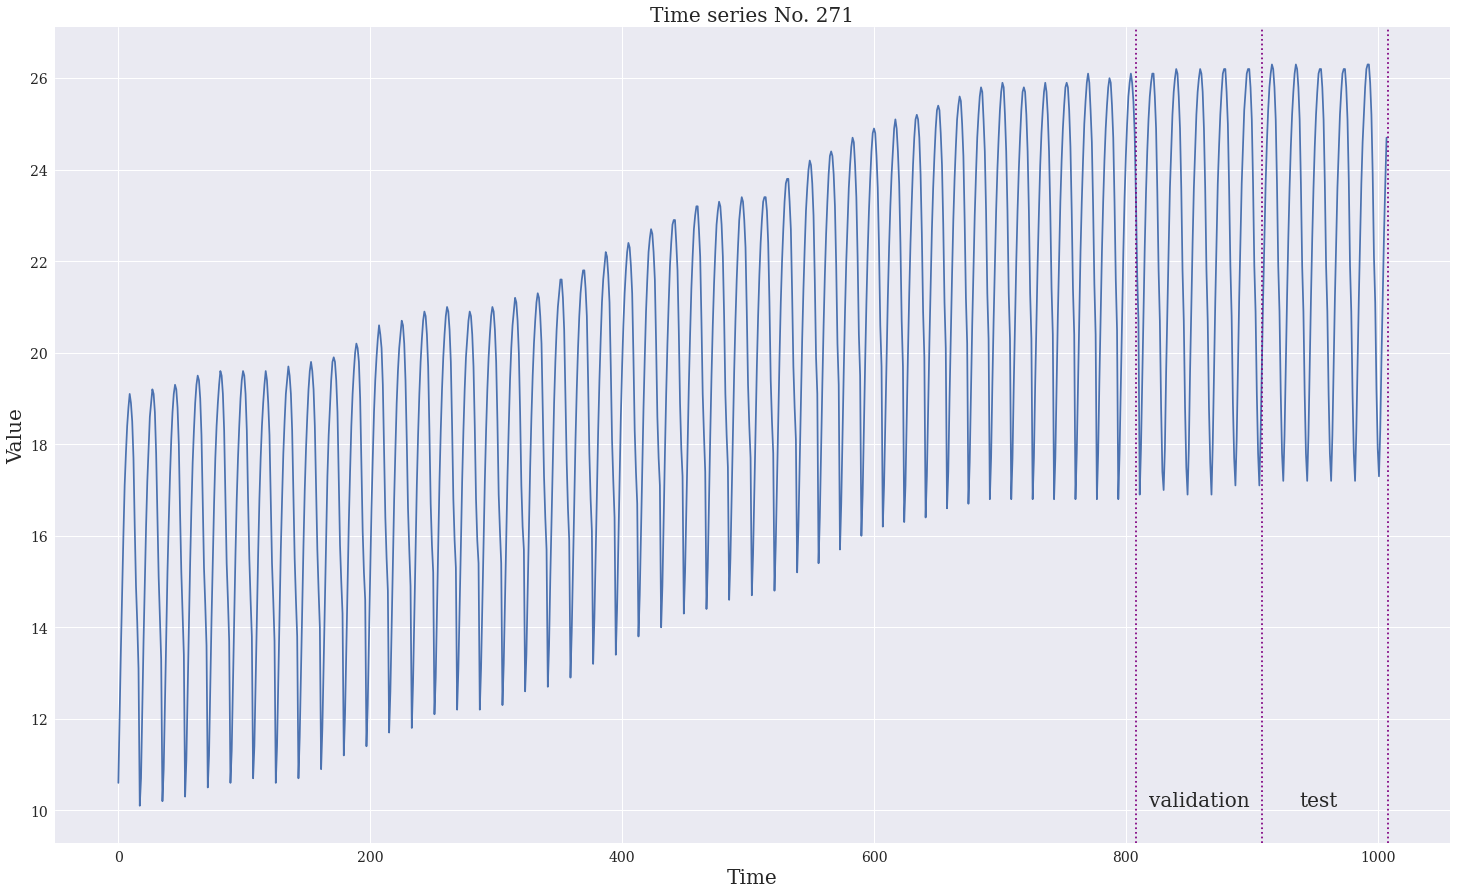
\includegraphics[width=\columnwidth]{hourly_271_ts}
    \caption{Time series No. 271 from M4 dataset}
    {\raggedright \footnotesize Time series No. 271 from M4 dataset is an hourly time series from unknown domain. We mark the segments used for validation (model selection) and testing.\par}
    \label{fig: hourly 271 ts}
\end{figure}
Figure \ref{fig: hourly 271 en} marks the predictions of EN on the test set of time series 271. We can see that although EN\_tran overreacts around the peaks, the reason of EN\_tran doing so well is that such cyclical dynamics spends long periods of time experiencing linear trends between a peak and another. And we already learned from the previous results that DCT helps following trends better. As to other models, Figure \ref{fig: hourly 271 lsvr} and \ref{fig: hourly 271 mlp} show that LSVR and MLP without DCT are following the blue line very well such that they are hard to outperform. LSVR\_raw can even forecast the upcoming turn when there is a peak ahead.
\begin{figure}[H]
    \centering
    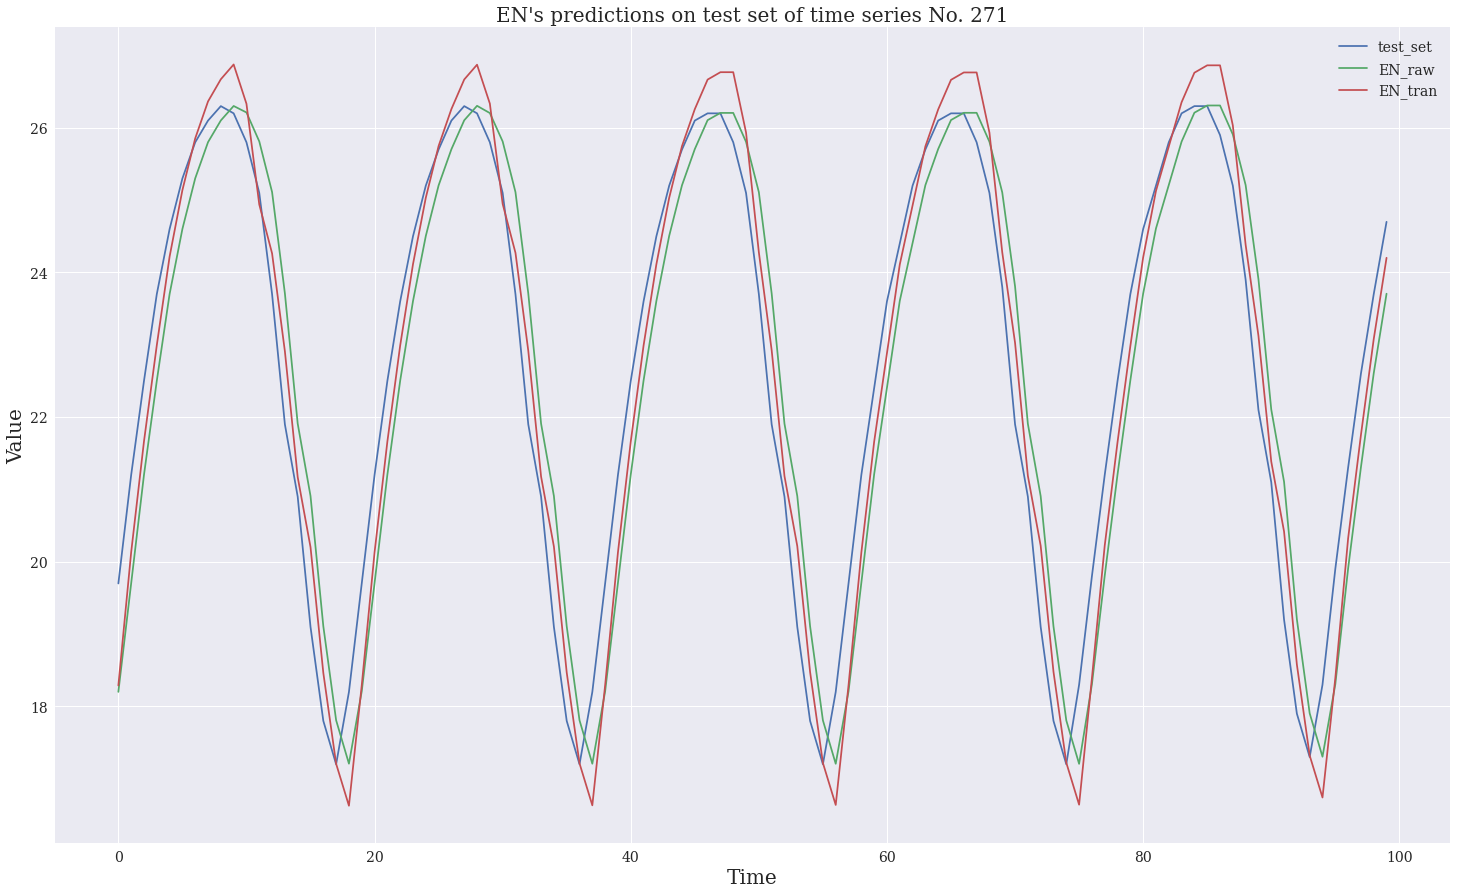
\includegraphics[width=\columnwidth]{hourly_271_en}
    \caption{EN on time series No. 271 from M4 dataset}
    {\raggedright \footnotesize This is EN's prediction on the test set of time series No. 271 from M4 dataset.  \par}
    \label{fig: hourly 271 en}
\end{figure}
\begin{figure}[H]
    \centering
    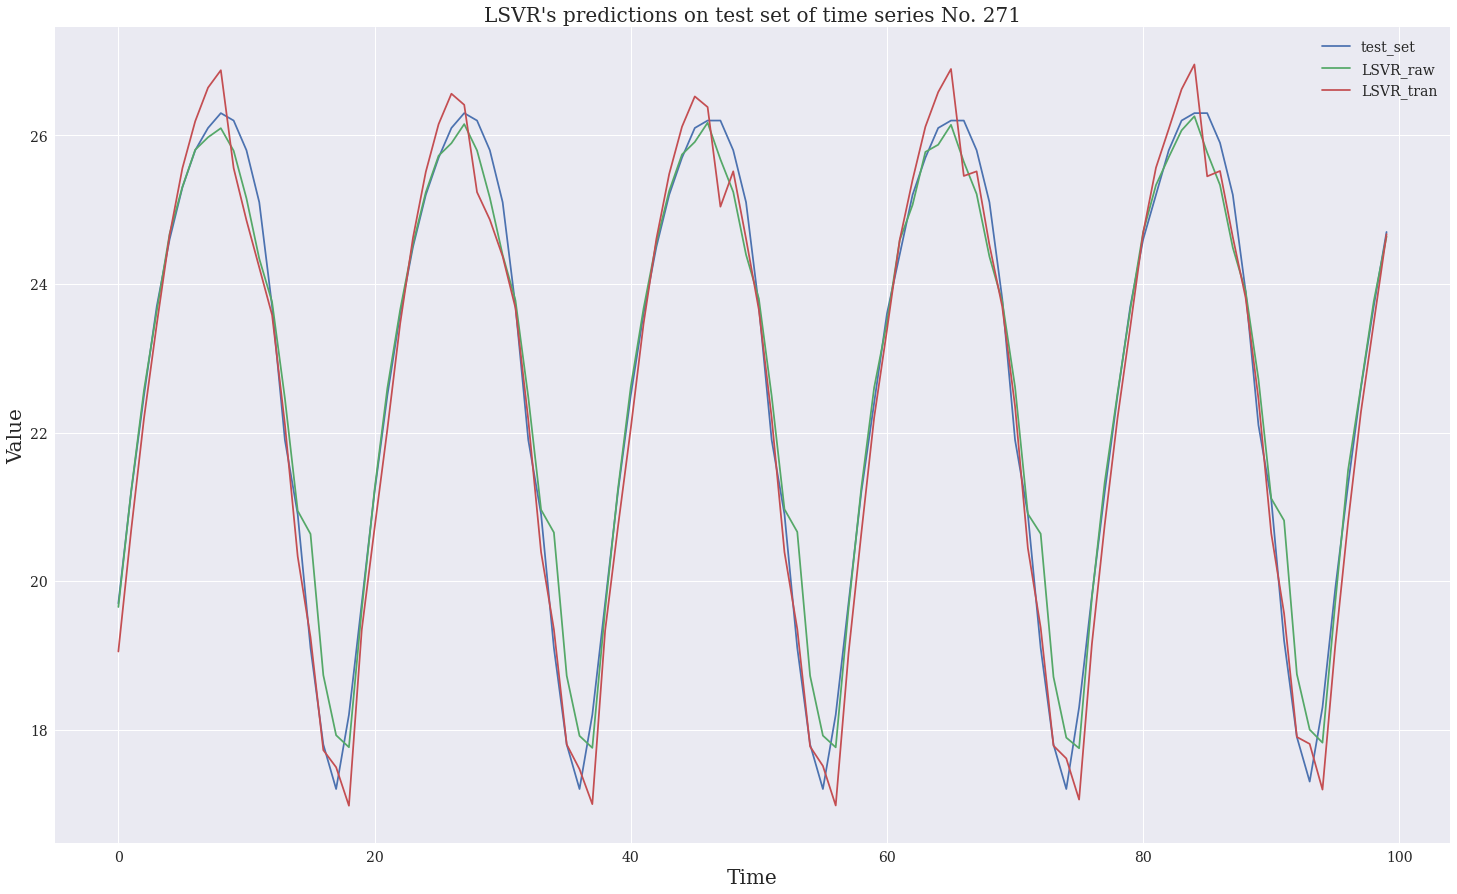
\includegraphics[width=\columnwidth]{hourly_271_lsvr}
    \caption{LSVR on time series No. 271 from M4 dataset}
    {\raggedright \footnotesize This is LSVR's prediction on the test set of time series No. 271 from M4 dataset.  \par}
    \label{fig: hourly 271 lsvr}
\end{figure}
\begin{figure}[H]
    \centering
    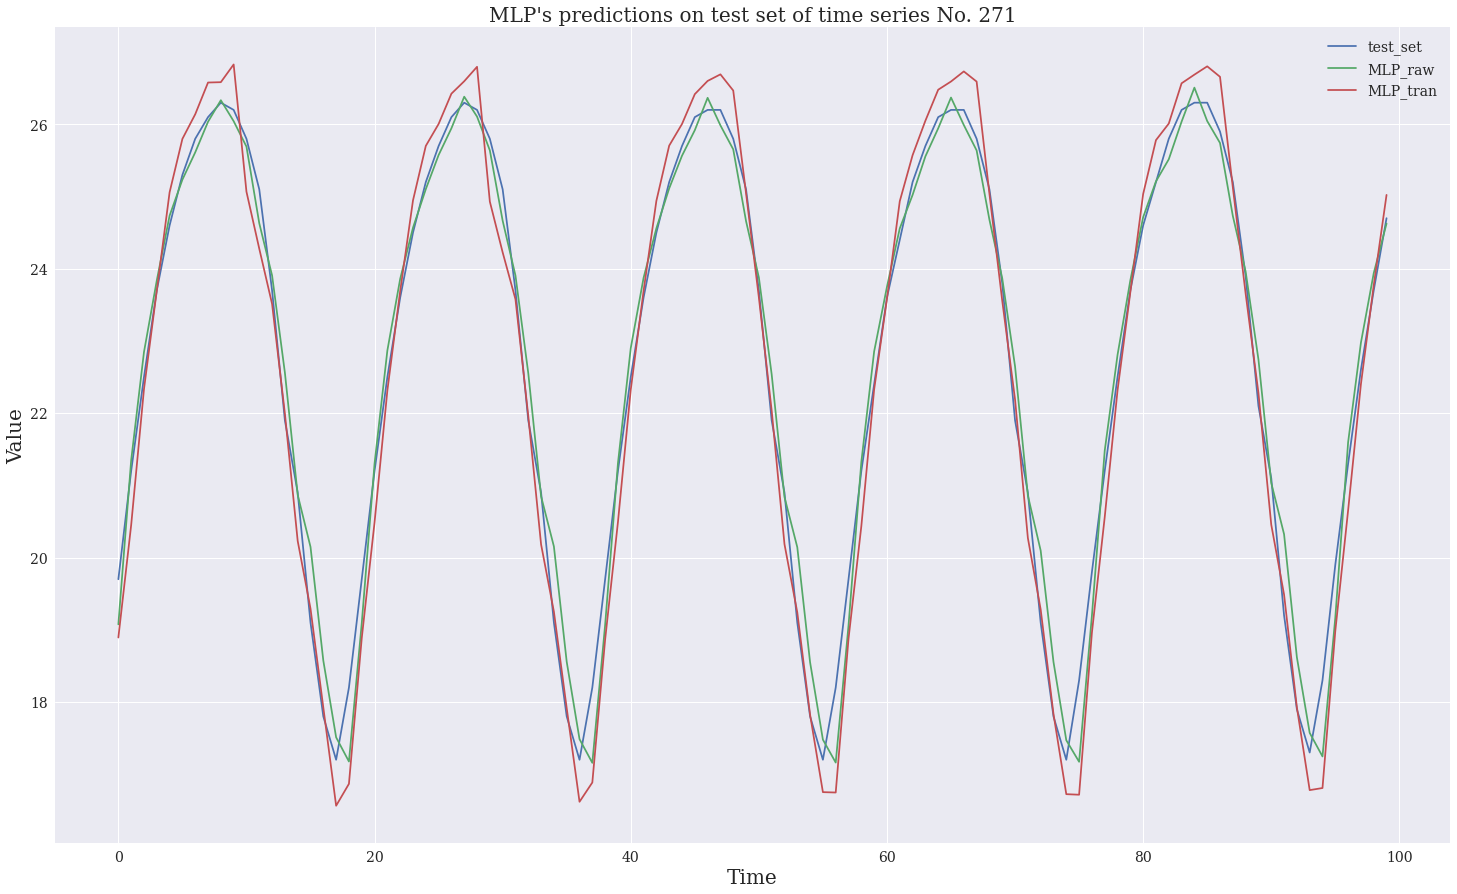
\includegraphics[width=\columnwidth]{hourly_271_mlp}
    \caption{MLP on time series No. 271 from M4 dataset}
    {\raggedright \footnotesize This is MLP's prediction on the test set of time series No. 271 from M4 dataset.  \par}
    \label{fig: hourly 271 mlp}
\end{figure}

\section{Discussion}
In our experiment, we trained models with and without DCT in all cases to investigate the features of DCT. However, in practice, applying DCT should be considered as an optional policy. One should set a hyperparameter that gives the model an opportunity to decide not to use DCT during model selection.

In general, we estimate that it can be worth it to try using DC Transformation in modelling tasks. DCT reduces noise where the interpretation has been applied. In comparison to most denoising/smoothing methods, DCT preserves the information carried by the peaks without toning them down. This gives DCT the ability to reduce noise while also capturing extreme events. Moreover, due to the interpolation being linear, DCT emphases the trend in the time series that can lead to better model performance. Seeing that interpolation does play an important role in DCT, we tried other interpolation methdos during exploratory trials. We tried quadratic and cubic interpolations that fit degree-two or degree-three polynomials in the intervals. We find both interpolation inadequate because they tend to create peaks in the intervals by their polynomial nature. However, the intervals are supposed to be smooth because the peaks are already captured by the DC algorithm. We tried another interpolation called Akima interpolation (Akima (\citeyear{akima1970new})). Akima interpolation is a middle point between linear and quadratic interpolation. We find it does perform better than quadratic interpolation, but we conclude that linear interpolation is still a better choice for our experiments.
